\documentclass[14pt]{extreport}
\usepackage{cmap}
\usepackage[utf8]{inputenc}
\usepackage[english,ukrainian]{babel}
\usepackage{graphicx}
\usepackage{geometry}
\usepackage{listings}
\usepackage{amsmath}
\usepackage{float}
\geometry{
	a4paper,
	left=20mm,
	right=20mm,
	top=20mm,
	bottom=20mm
}
\lstset{
	language=bash,
	tabsize=4,
	breaklines,
	keepspaces,
	showstringspaces=false,
}
\graphicspath{ {./pictures} }
\setlength{\parindent}{4em}

\newcommand\subject{Бази даних}
\newcommand\lecturer{асистент кафедри ПЗ\\Білоіваненко М.В.}
\newcommand\teacher{асистент кафедри ПЗ\\Майхер В.Ю.}
\newcommand\mygroup{ПЗ-32}
\newcommand\lab{2}
\newcommand\theme{Cтворення бази даних засобами графічного інтерфейсу програми PgAdmin}
\newcommand\purpose{творення бази даних засобами графічного інтерфейсу програми PgAdmin: створення таблиць, створення зв’язків між таблицями.}

\begin{document}
\begin{normalsize}
	\begin{titlepage}
		\thispagestyle{empty}
		\begin{center}
			\textbf{МІНІСТЕРСТВО ОСВІТИ І НАУКИ УКРАЇНИ\\
				НАЦІОНАЛЬНИЙ УНІВЕРСИТЕТ "ЛЬВІВСЬКА ПОЛІТЕХНІКА"}
		\end{center}
		\begin{flushright}
			Інститут \textbf{КНІТ}\\
			Кафедра \textbf{ПЗ}
		\end{flushright}
		\vspace{200pt}
		\begin{center}
			\textbf{ЗВІТ}\\
			\vspace{10pt}
			До лабораторної роботи № \lab\\
			\textbf{На тему}: “\textit{\theme}”\\
			\textbf{З дисципліни}: “\subject”
		\end{center}
		\vspace{40pt}
		\begin{flushright}
			
			\textbf{Лектор}:\\
			\lecturer\\
			\vspace{10pt}
			\textbf{Виконав}:\\
			
			студент групи \mygroup\\
			Коваленко Д.М.\\
			\vspace{10pt}
			\textbf{Прийняв}:\\
			
			\teacher\\
			
			\vspace{28pt}
			«\rule{1cm}{0.15mm}» \rule{1.5cm}{0.15mm} 2023 р.\\
			$\sum$ = \rule{1cm}{0.15mm}……………\\
			
		\end{flushright}
		\vspace{\fill}
		\begin{center}
			\textbf{Львів — 2023}
		\end{center}
	\end{titlepage}
		
	\begin{description}
		\item[Тема.] \theme.
		\item[Мета.] \purpose.
	\end{description}

	\section*{Лабораторне завдання}
	\begin{enumerate}
		\item В СУБД PostgreSQL створити навчальну базу даних "Операції купівлі-продажу". Назва бази даних повинна містити прізвище власника.
		\item В СУБД PostreSQL за допомогою графічного інтерфейсу створити таблиці бази даних "Операції купівлі-продажу" та базу даних індивідуального завдання.
		\item В СУБД PostgreSQL за допомогою графічного інтерфейсу побудувати діаграму бази даних "Операції купівлі-продажу" та базу даних індивідуального завдання.
		\item Оформити звіт.
	\end{enumerate}
	
	\section*{Хід роботи}
	\subsection*{База даних "Операції купівлі-продажу"}
	\iffalse
	\begin{figure}[H]
		\centering
		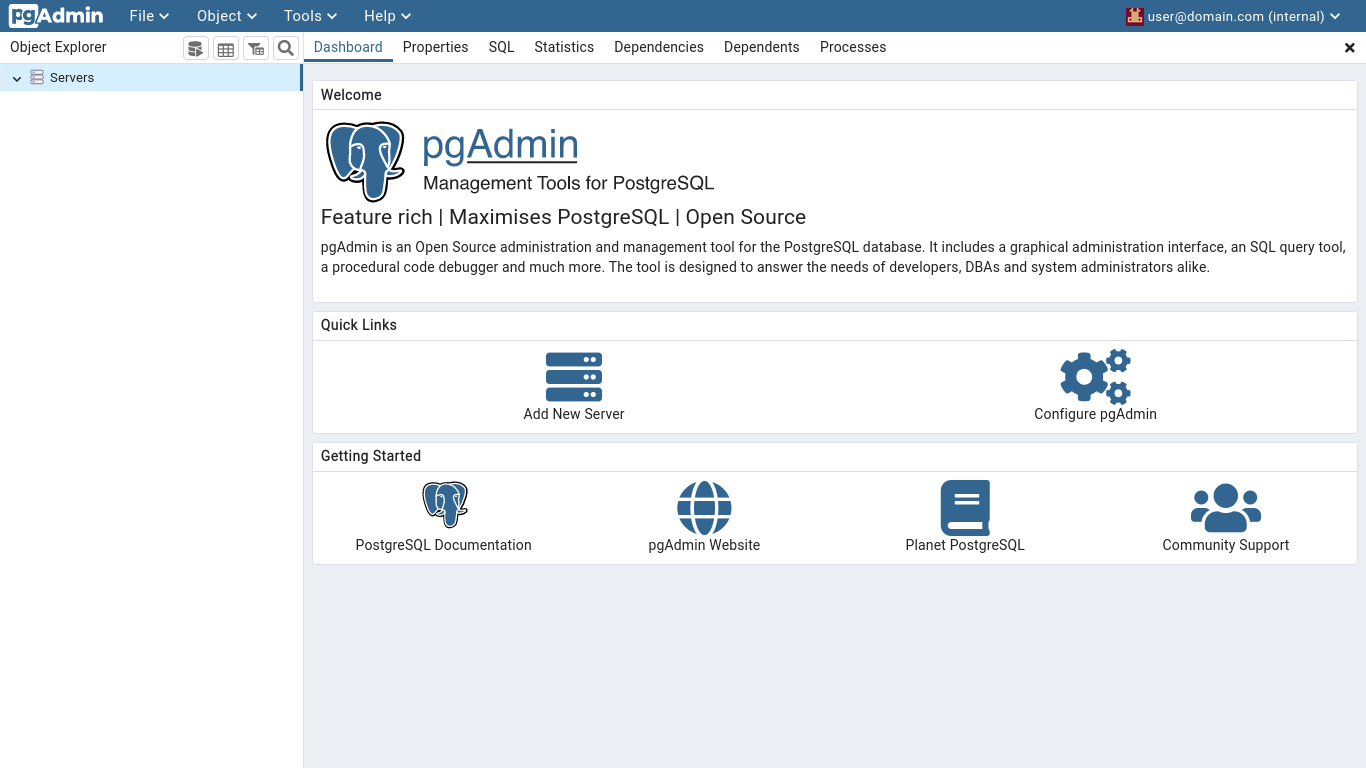
\includegraphics[scale=0.35]{1}
		\caption{Головна сторінка PgAdmin}
	\end{figure}

	\begin{figure}[H]
		\centering
		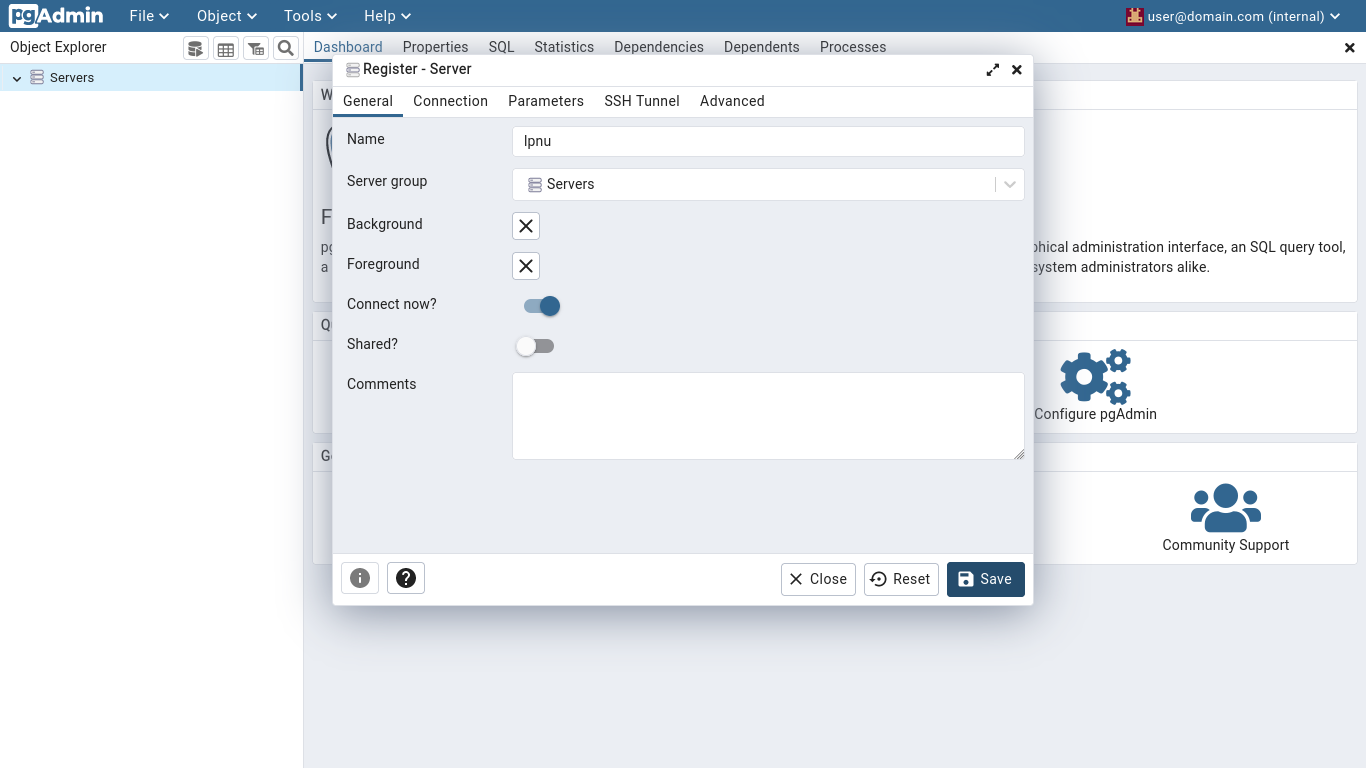
\includegraphics[scale=0.35]{2}
		\caption{Під'єднання до сервера PostgreSQL}
	\end{figure}
	
	\begin{figure}[H]
		\centering
		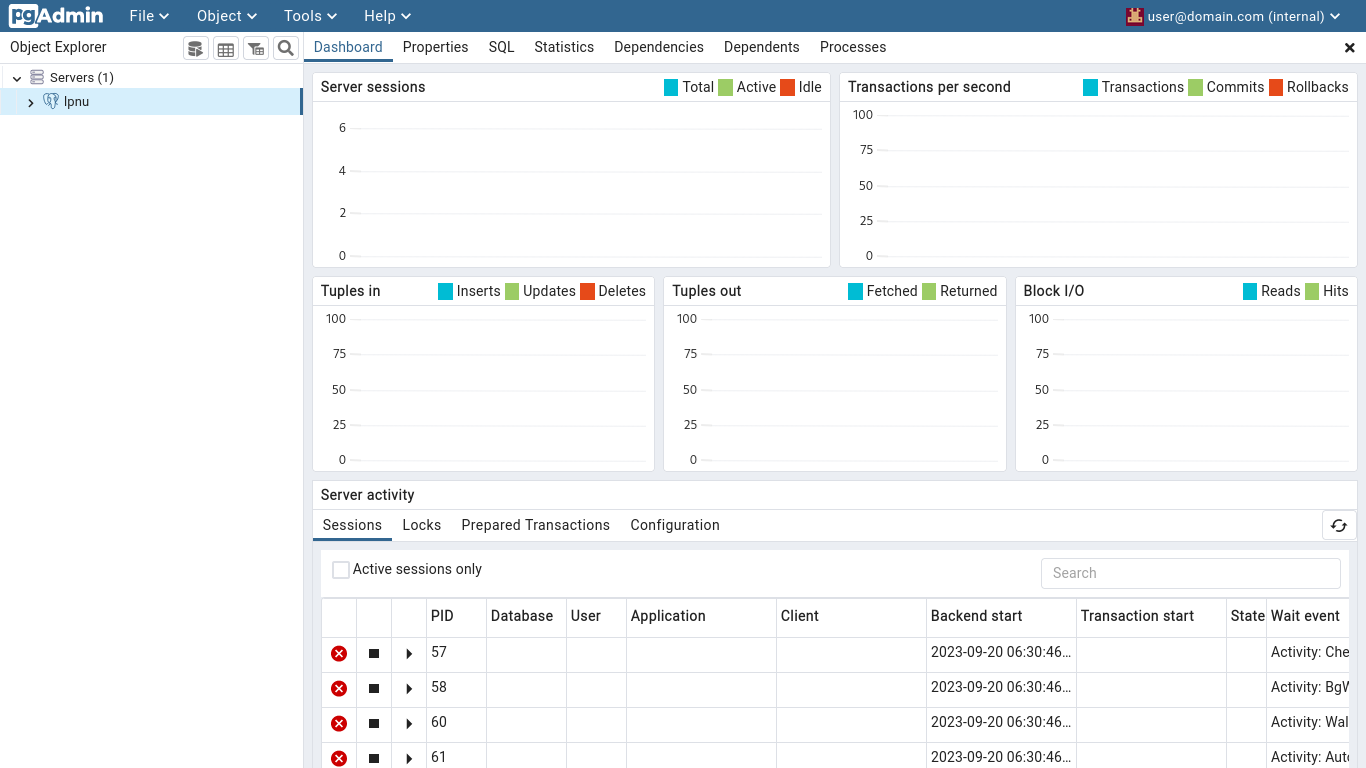
\includegraphics[scale=0.35]{3}
		\caption{Сторінка огляду сервера PostgreSQL}
	\end{figure}
	
	\begin{figure}[H]
		\centering
		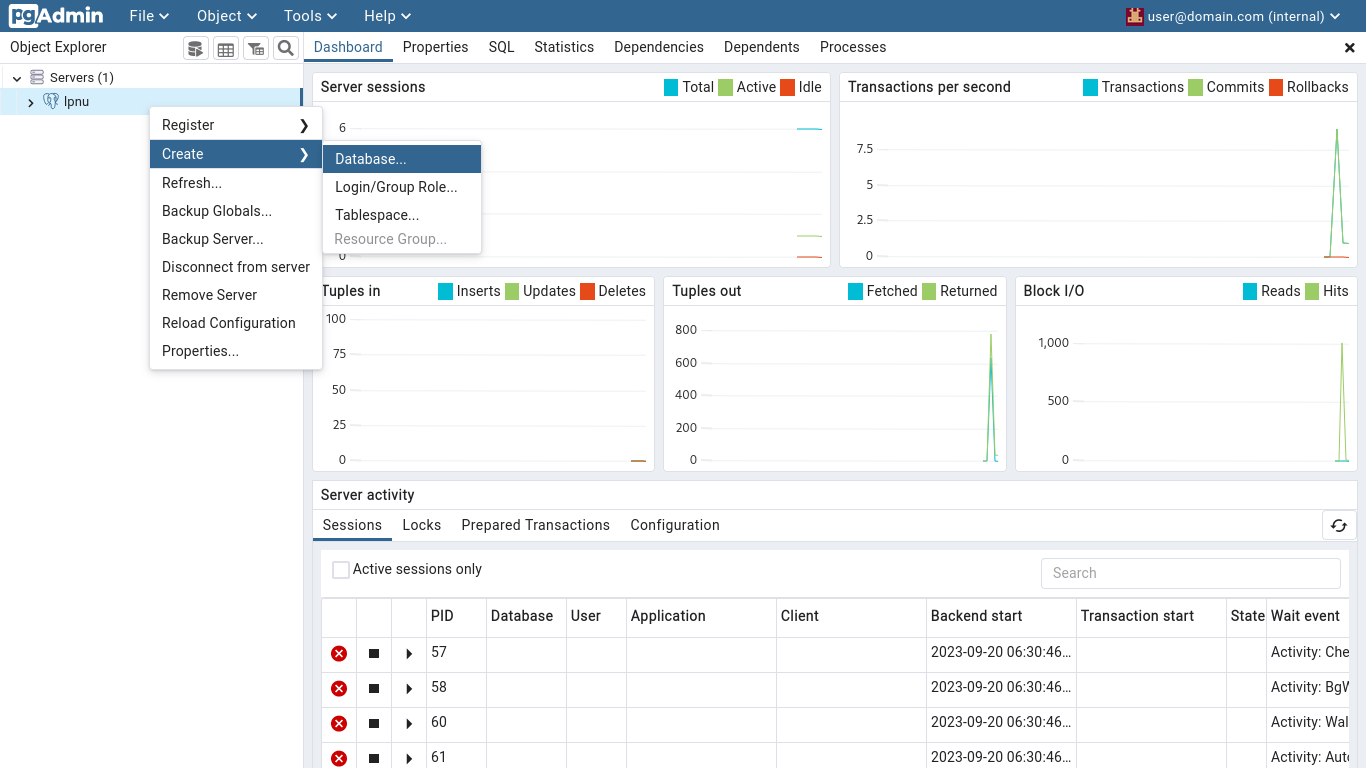
\includegraphics[scale=0.35]{4}
		\caption{Створення бази даних}
	\end{figure}
	
	\begin{figure}[H]
		\centering
		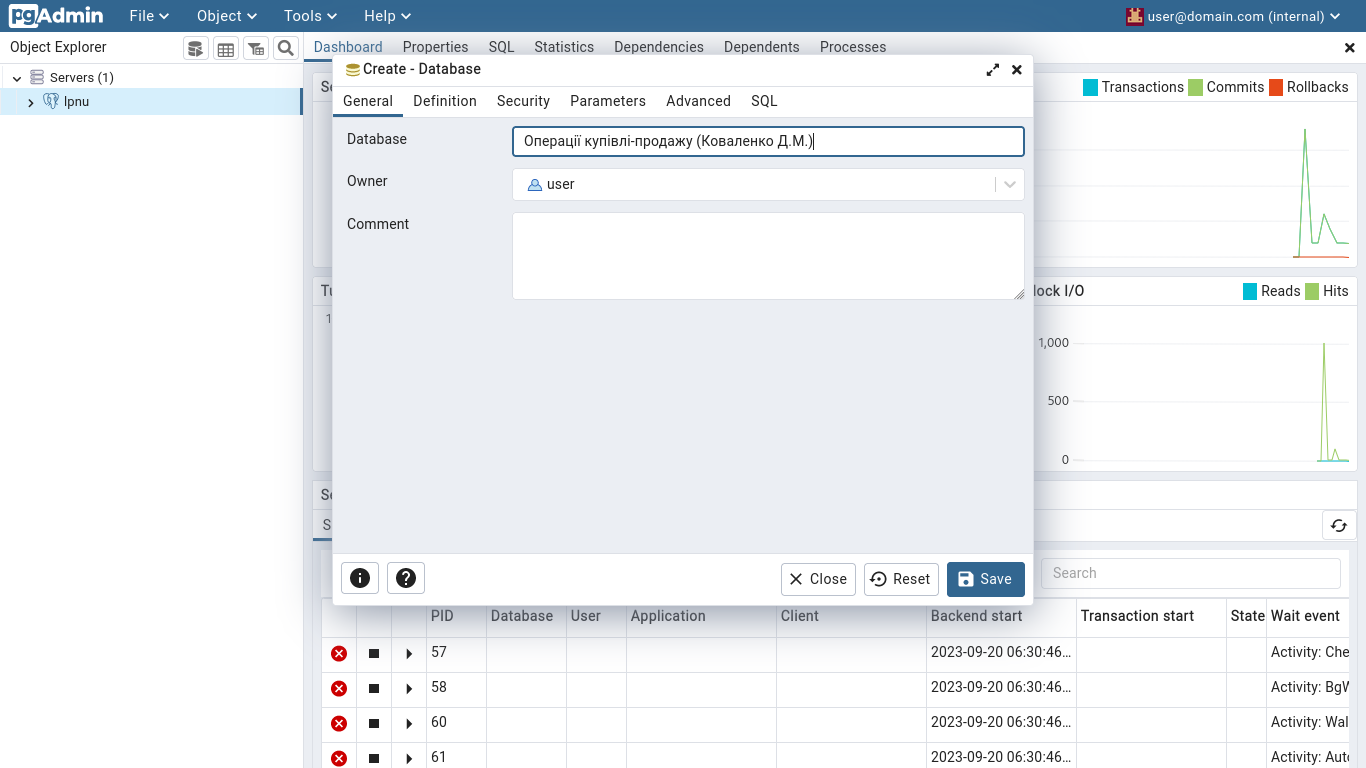
\includegraphics[scale=0.35]{5}
		\caption{Створення бази даних}
	\end{figure}
	
	\begin{figure}[H]
		\centering
		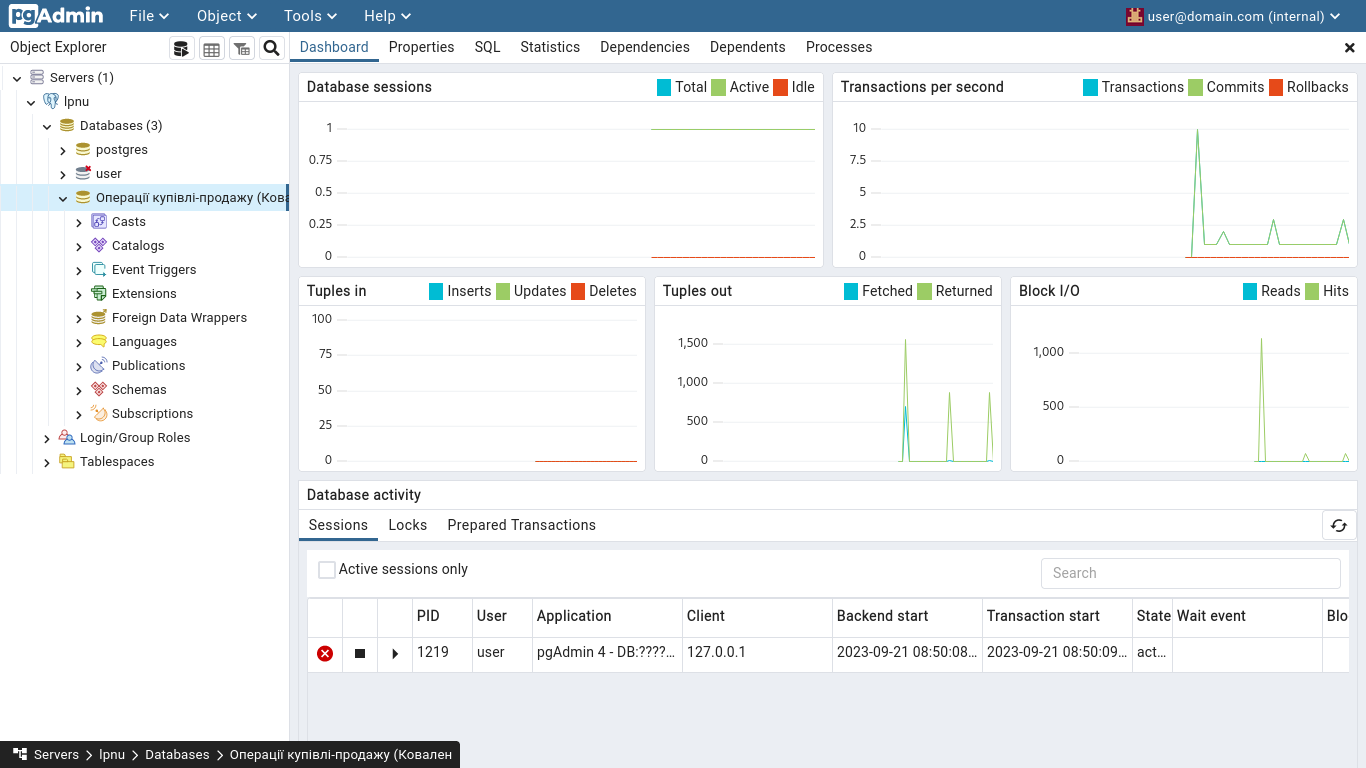
\includegraphics[scale=0.35]{7}
		\caption{Сторінка огляду бази даних}
	\end{figure}
	
	\begin{figure}[H]
		\centering
		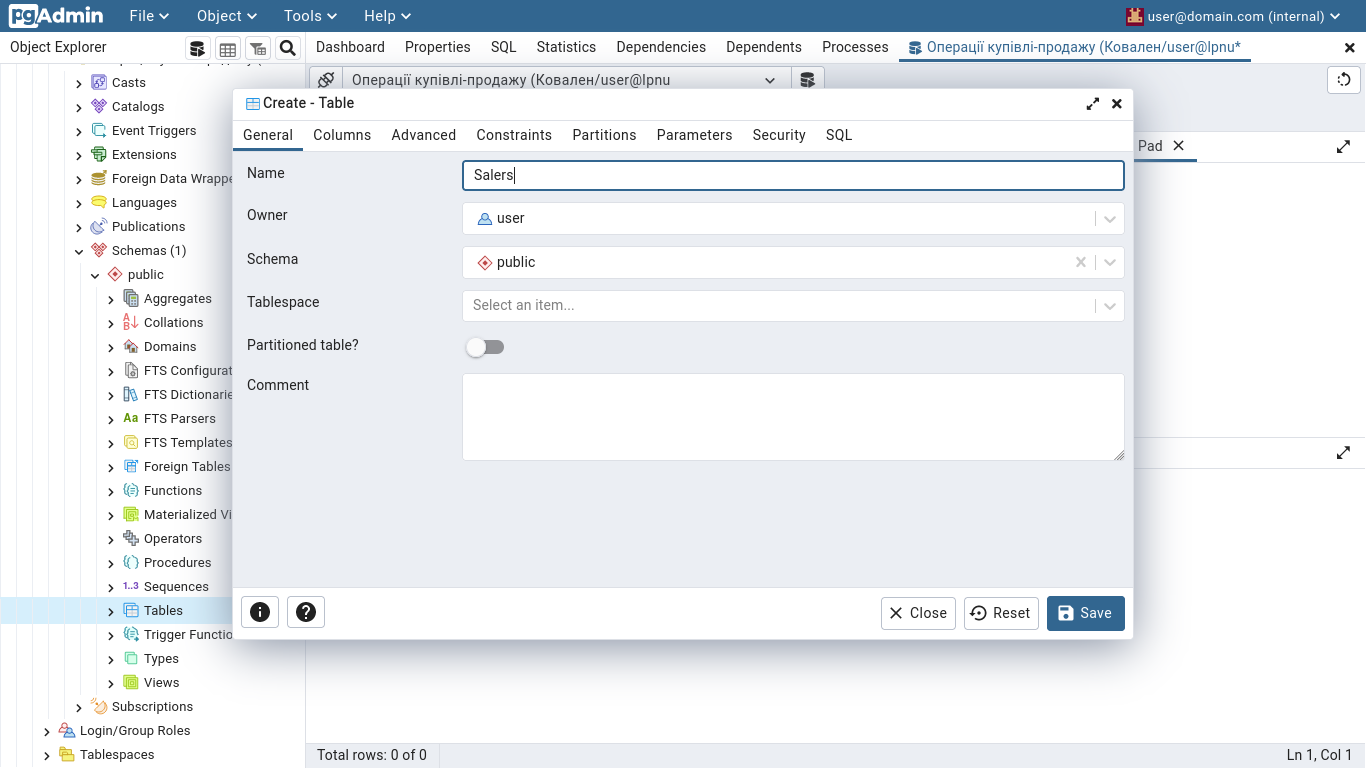
\includegraphics[scale=0.35]{8}
		\caption{Створення таблиці Salers}
	\end{figure}
	
	\begin{figure}[H]
		\centering
		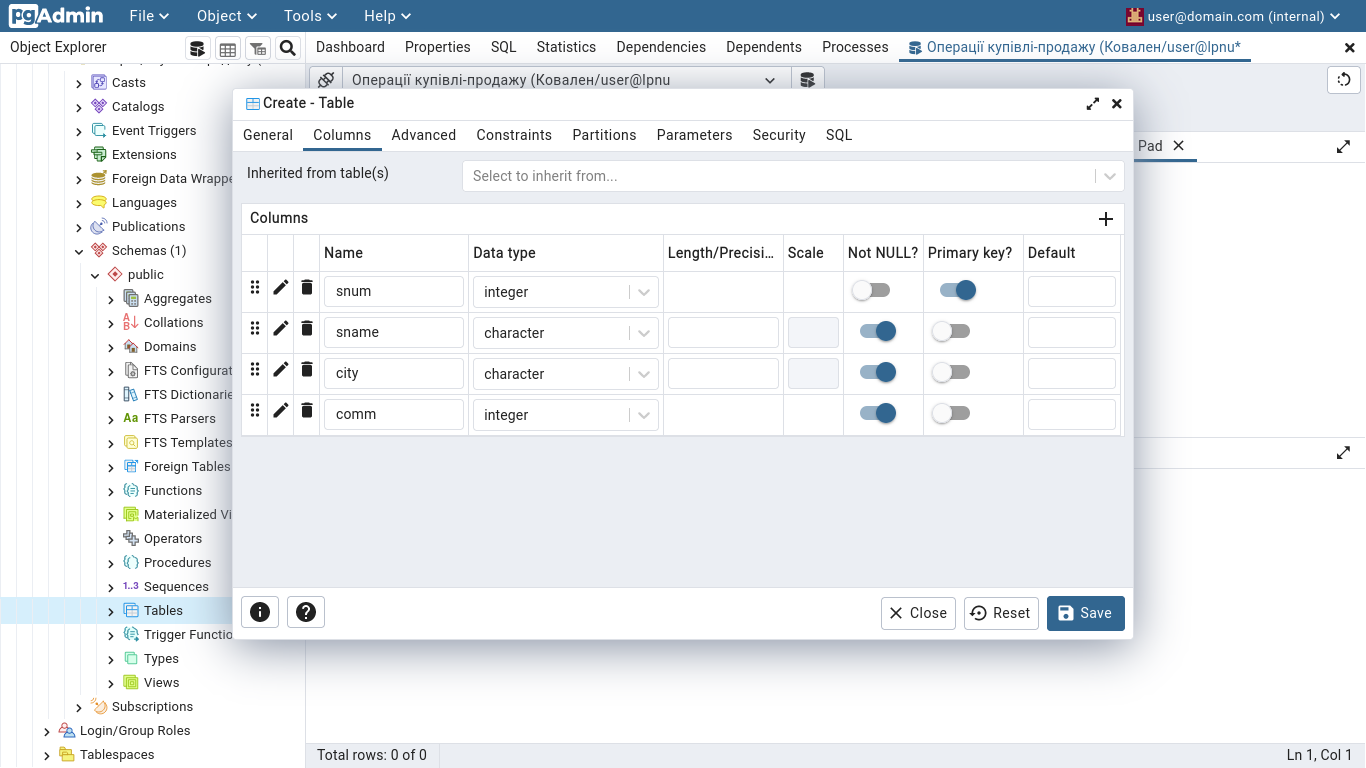
\includegraphics[scale=0.35]{9}
		\caption{Створення полів таблиці Salers}
	\end{figure}
	
	\begin{figure}[H]
		\centering
		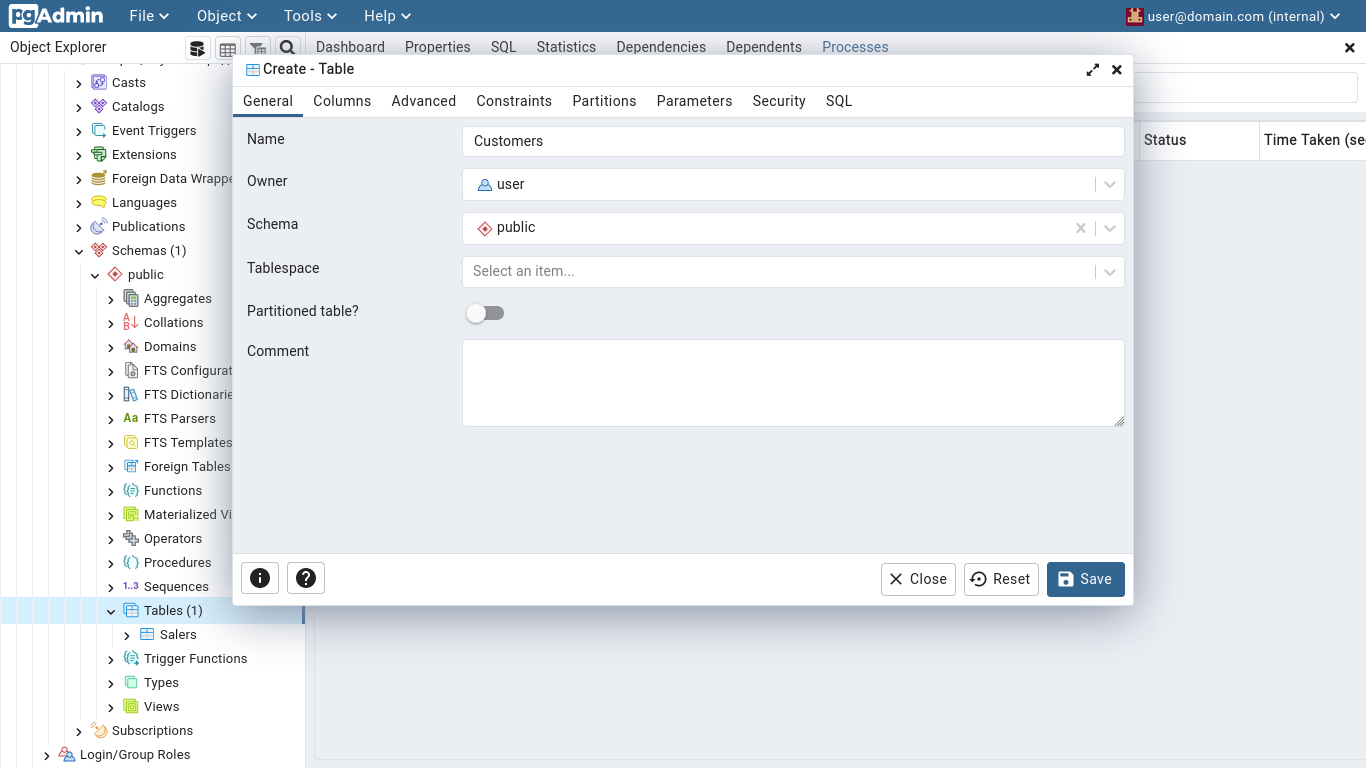
\includegraphics[scale=0.35]{10}
		\caption{Створення таблиці Customers}
	\end{figure}
	
	\begin{figure}[H]
		\centering
		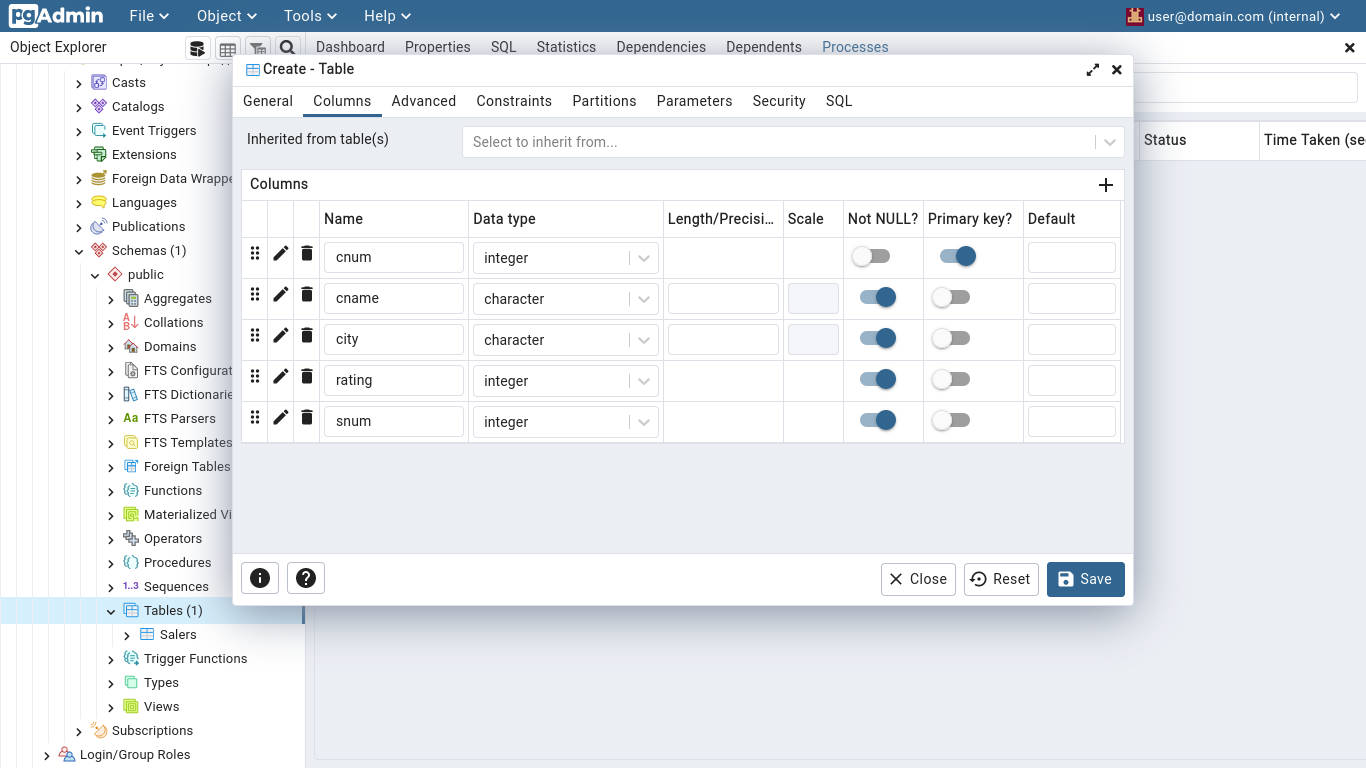
\includegraphics[scale=0.35]{11}
		\caption{Створення полів таблиці Customers}
	\end{figure}
	
	\begin{figure}[H]
		\centering
		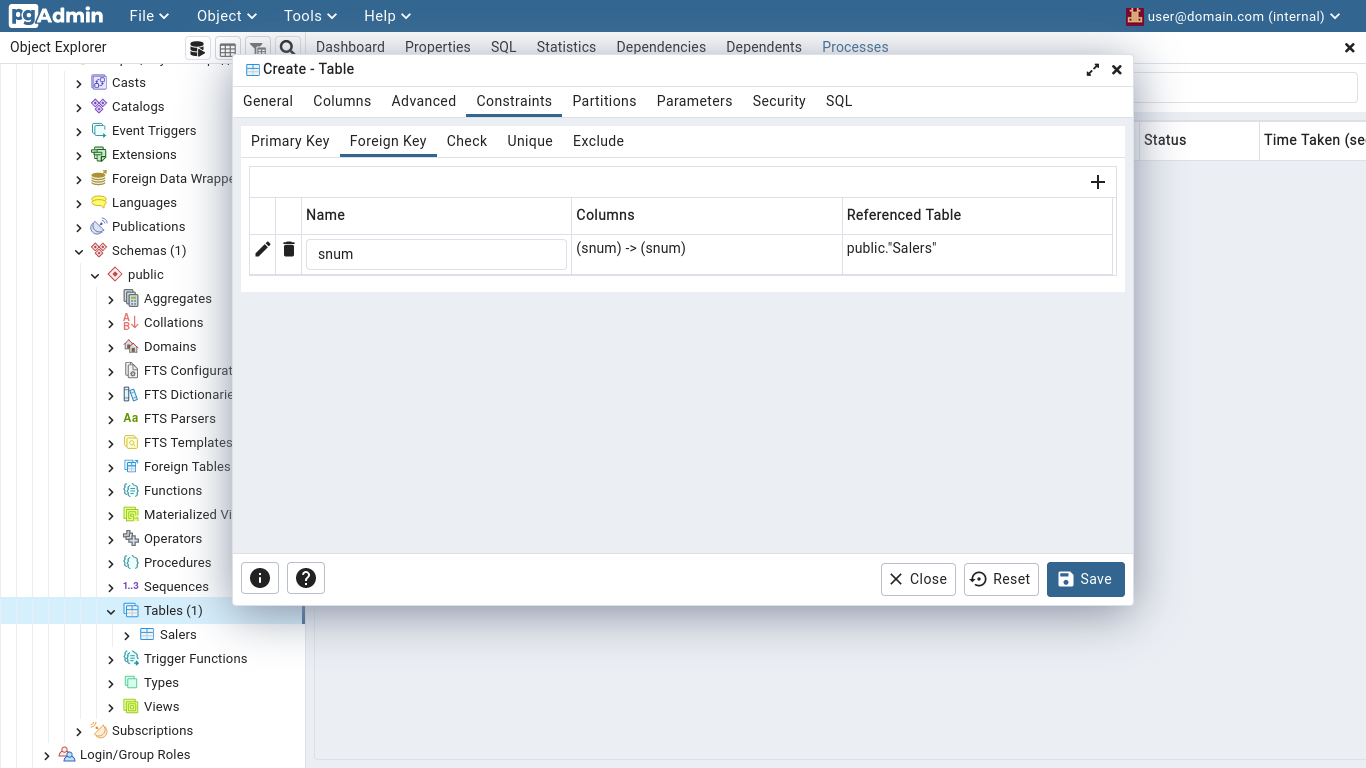
\includegraphics[scale=0.35]{12}
		\caption{Створення полів таблиці Customers}
	\end{figure}
	
	\begin{figure}[H]
		\centering
		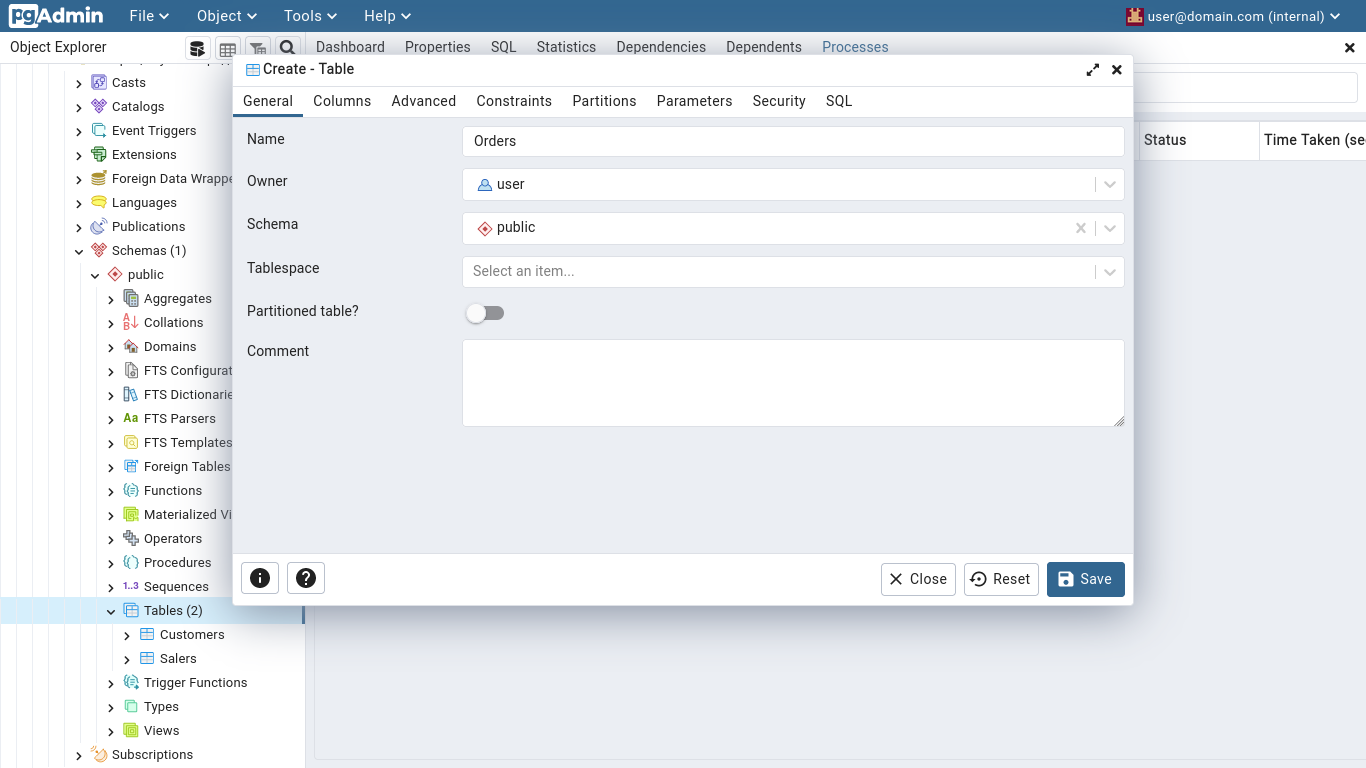
\includegraphics[scale=0.35]{13}
		\caption{Створення таблиці Orders}
	\end{figure}
	
	\begin{figure}[H]
		\centering
		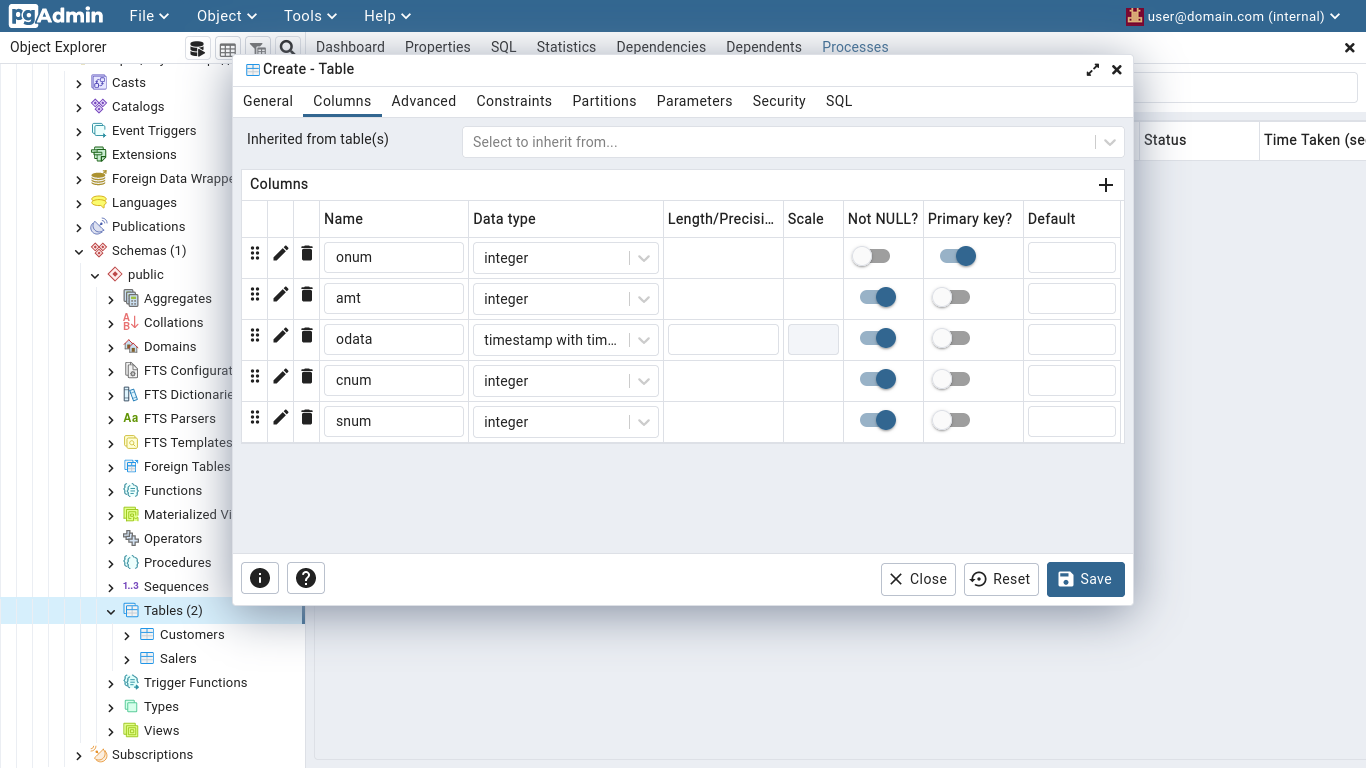
\includegraphics[scale=0.35]{14}
		\caption{Створення полів таблиці Orders}
	\end{figure}
	
	\begin{figure}[H]
		\centering
		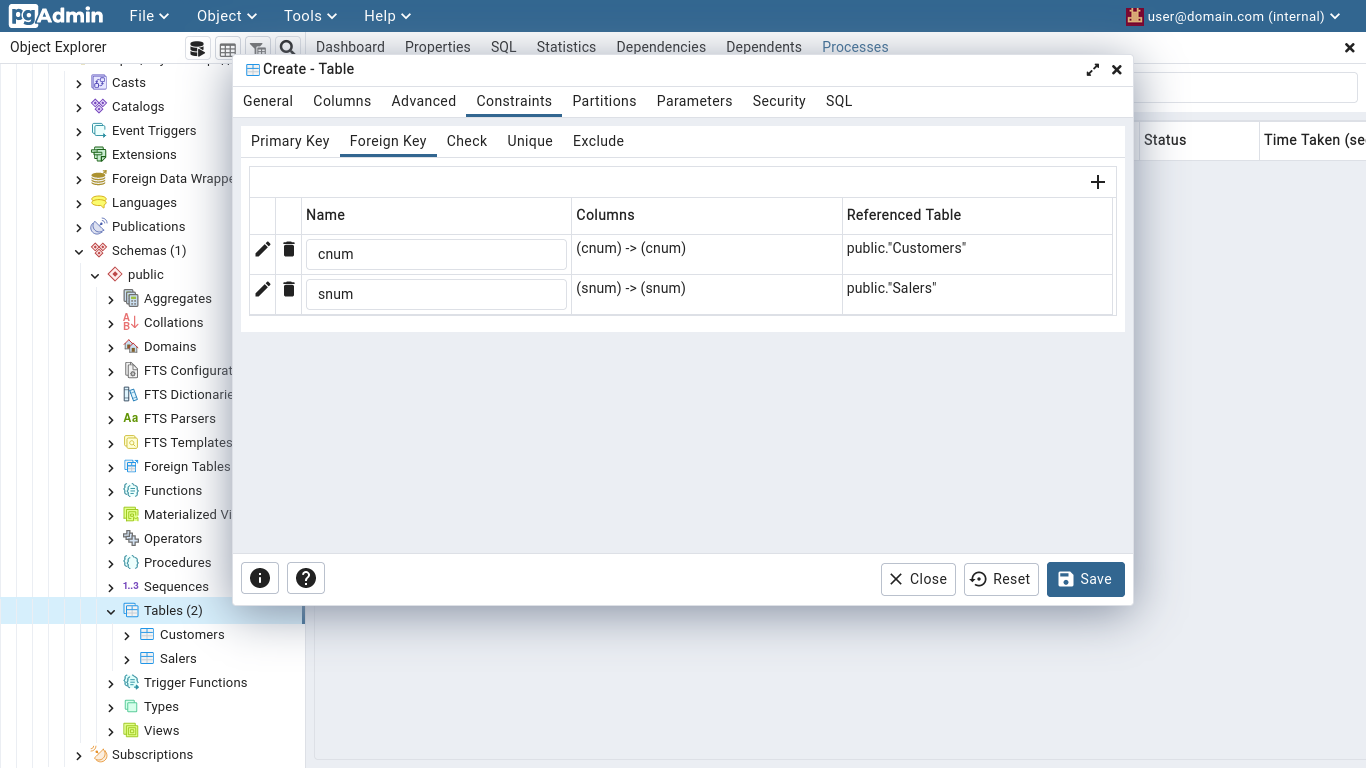
\includegraphics[scale=0.35]{15}
		\caption{Створення полів таблиці Orders}
	\end{figure}
	\fi
	\begin{figure}[H]
		\centering
		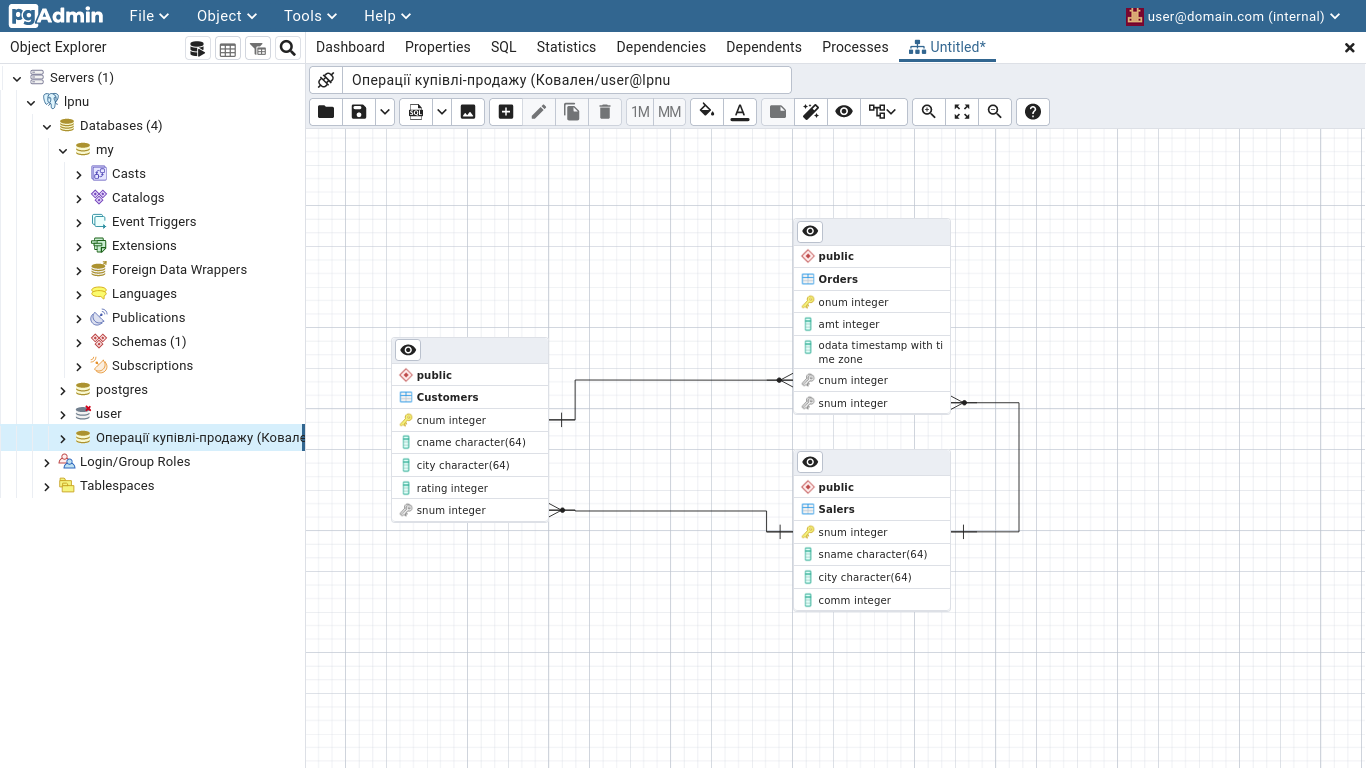
\includegraphics[scale=0.35]{16}
		\caption{Діаграма бази даних "Операції купівлі-продажу"}
	\end{figure}

	\subsection*{База даних індивідуального завдання}
	\textbf{Варіант}: база даних для роботи компанії з регулярних перевезень пасажирів.
	
	\noindent\textbf{Опис бізнес процесів:}
	\begin{enumerate}
		\item Можливість відслідковування транспорту на маршрутах.
		\item Автоматизація процесу продажу та перевірки квитків.
	\end{enumerate}

	\noindent\textbf{Опис бази даних:}
	\begin{itemize}
		\item \textbf{timetable} (\textit{id}, \textit{route\_id}, \textit{vehicle\_id}, \textit{departure\_time}, \textit{arrival\_time}, \textit{price}):
		\begin{itemize}
			\item \textbf{id} - унікальний номер транспортного засобу;
			\item \textbf{route\_id} - посилання на номер маршруту;
			\item \textbf{vehicle\_id} - посилання на номер транспортного засобу;
			\item \textbf{departure\_time} - час відправлення;
			\item \textbf{arrival\_time} - час прибуття;
			\item \textbf{price} - вартість квитка;
		\end{itemize}
		\item \textbf{route} (\textit{id}, \textit{name}, \textit{distance}):
		\begin{itemize}
			\item \textbf{id} - унікальний номер маршруту;
			\item \textbf{name} - назва маршруту;
			\item \textbf{distance} - протяжність маршруту;
		\end{itemize}
		\item \textbf{stop} (\textit{id}, \textit{name}, \textit{coords}):
		\begin{itemize}
			\item \textbf{id} - унікальний номер зупинки;
			\item \textbf{name} - назва зупинки;
			\item \textbf{coords} - геогерафічні координати зупинки;
		\end{itemize}
		\item \textbf{route\_stop} (\textit{id}, \textit{route\_id}, \textit{stop\_id}, \textit{order\_index}):
		\begin{itemize}
			\item \textbf{id} - унікальний номер запису;
			\item \textbf{route\_id} -  посилання на номер маршруту;
			\item \textbf{stop\_id} - посилання на номер зупинки;
			\item \textbf{order\_index} - порядковий номер зупинки на маршруті;
		\end{itemize}
		\item \textbf{vehicle} (\textit{id}, \textit{type}, \textit{status}, \textit{route\_id}, \textit{coords}, \textit{license\_plate}, \textit{capacity}):
		\begin{itemize}
			\item \textbf{id} - унікальний номер транспортного засобу;
			\item \textbf{type} - тип транспортного засобу; 
			\item \textbf{status} - статус транспортного засобу (в дорозі, в обслуговування, інше);
			\item \textbf{route\_id} - посилання на номер маршруту;
			\item \textbf{coords} - географічні координати транспортного засобу на маршруті;
			\item \textbf{license\_plate} - номерний знак транспортного засобу;
			\item \textbf{capacity} - місткість транспортного засобу;
		\end{itemize}
		\item \textbf{passenger} (\textit{id}, \textit{name}, \textit{email}, \textit{password}):
		\begin{itemize}
			\item \textbf{id} - унікальний номер пасажира;
			\item \textbf{name} - ім'я пасажира;
			\item \textbf{email} - електронна пошта пасажира;
			\item \textbf{password} - пароль пасажира;
		\end{itemize}
		\item \textbf{feedback} (\textit{id}, \textit{passenger\_id}, \textit{time}, \textit{message}):
		\begin{itemize}
			\item \textbf{id} - унікальний номер повідомлення;
			\item \textbf{passenger\_id} - посилання на номер пасажира;
			\item \textbf{time} - час повідомлення;
			\item \textbf{message} - текст повідомлення;
		\end{itemize}
		\item \textbf{ticket} (\textit{id}, \textit{passenger\_id}, \textit{timetable\_id}, \textit{purchase\_time}, \textit{seat}):
		\begin{itemize}
			\item \textbf{id} - унікальний номер квитка;
			\item \textbf{passenger\_id} - посилання на пасажира;
			\item \textbf{timetable\_id} - посилання на номер запису у розкладі;
			\item \textbf{purchase\_time} - час покупки;
			\item \textbf{seat} - номер сидіння;
		\end{itemize}
		\item \textbf{driver} (\textit{id}, \textit{name}, \textit{vehicle\_id}):
		\begin{itemize}
			\item \textbf{id} - унікальний номер транспортного засобу;
			\item \textbf{vehicle\_id} - посилання на номер транспортного засобу;
			\item \textbf{name} - ім'я водія;
		\end{itemize}
		\item \textbf{maintenance\_log} (\textit{id}, \textit{vehicle\_id}, \textit{time}, \textit{description}, \textit{cost});
		\begin{itemize}
			\item \textbf{id} - унікальний номер запису про обслуговування;
			\item \textbf{vehicle\_id} - посилання на номер транспортного засобу;
			\item \textbf{time} - час проведення обслуговування;
			\item \textbf{description} - опис обслуговування;
			\item \textbf{cost} - вартість обслуговування;
		\end{itemize}
	\end{itemize}
	
	
	\begin{figure}[H]
		\centering
		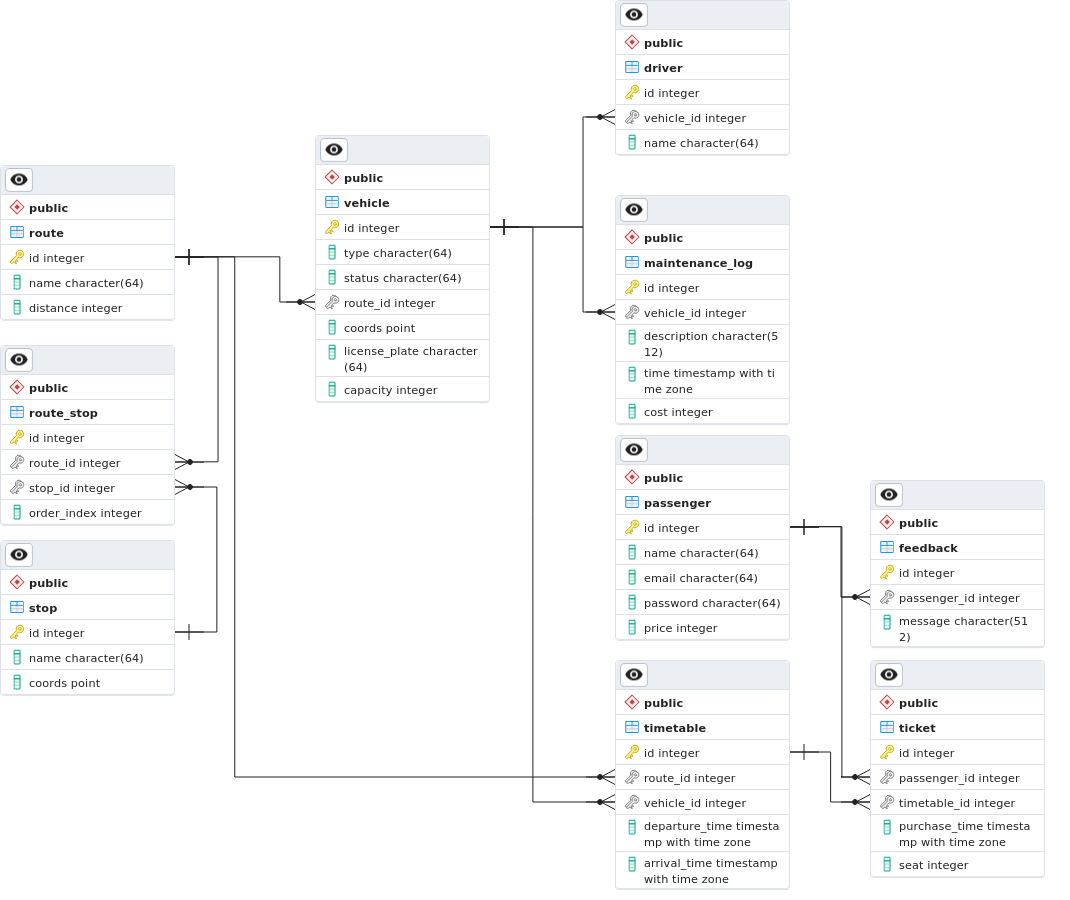
\includegraphics[scale=0.4]{50}
		\caption{Діаграма бази даних індивідуального варіанту}
	\end{figure}
	
	\iffalse
	\begin{figure}[H]
		\centering
		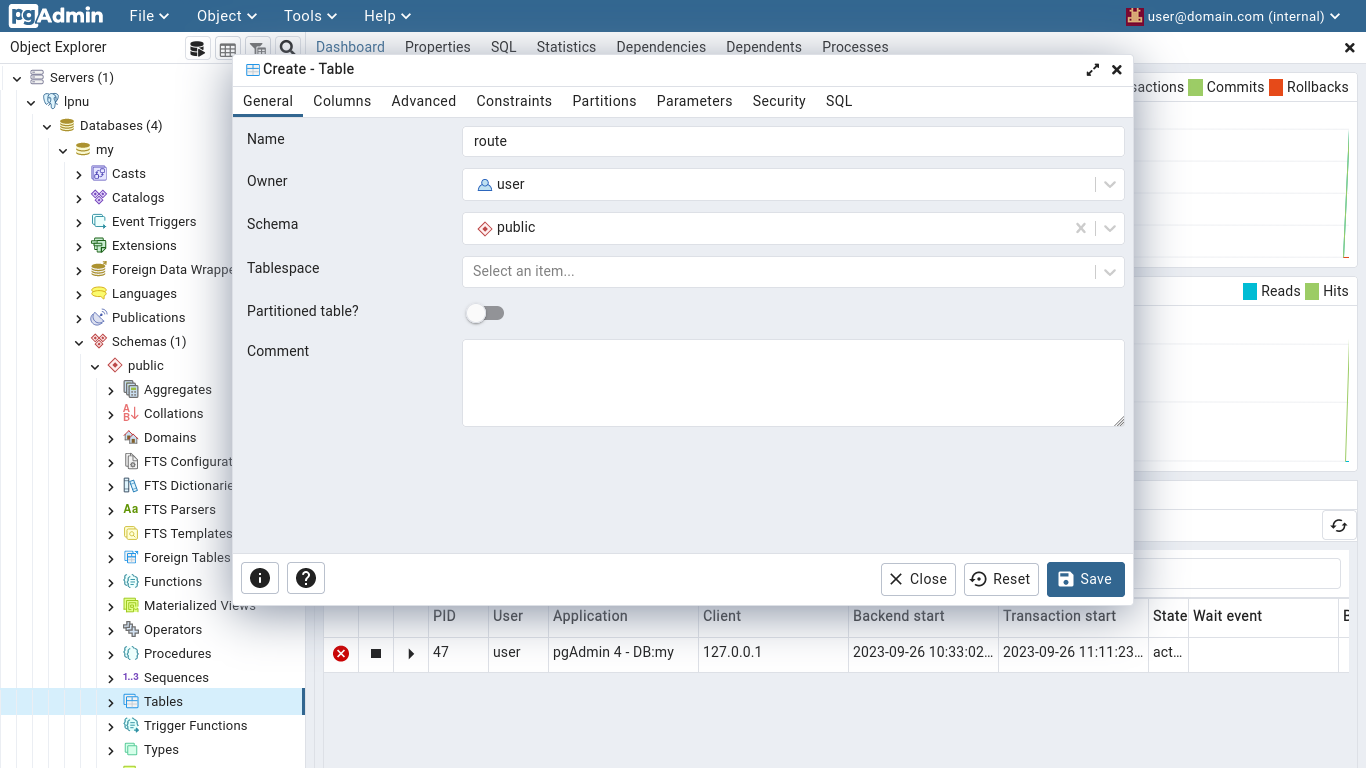
\includegraphics[scale=0.35]{20}
		\caption{Створення таблиці "route"}
	\end{figure}
	
	\begin{figure}[H]
		\centering
		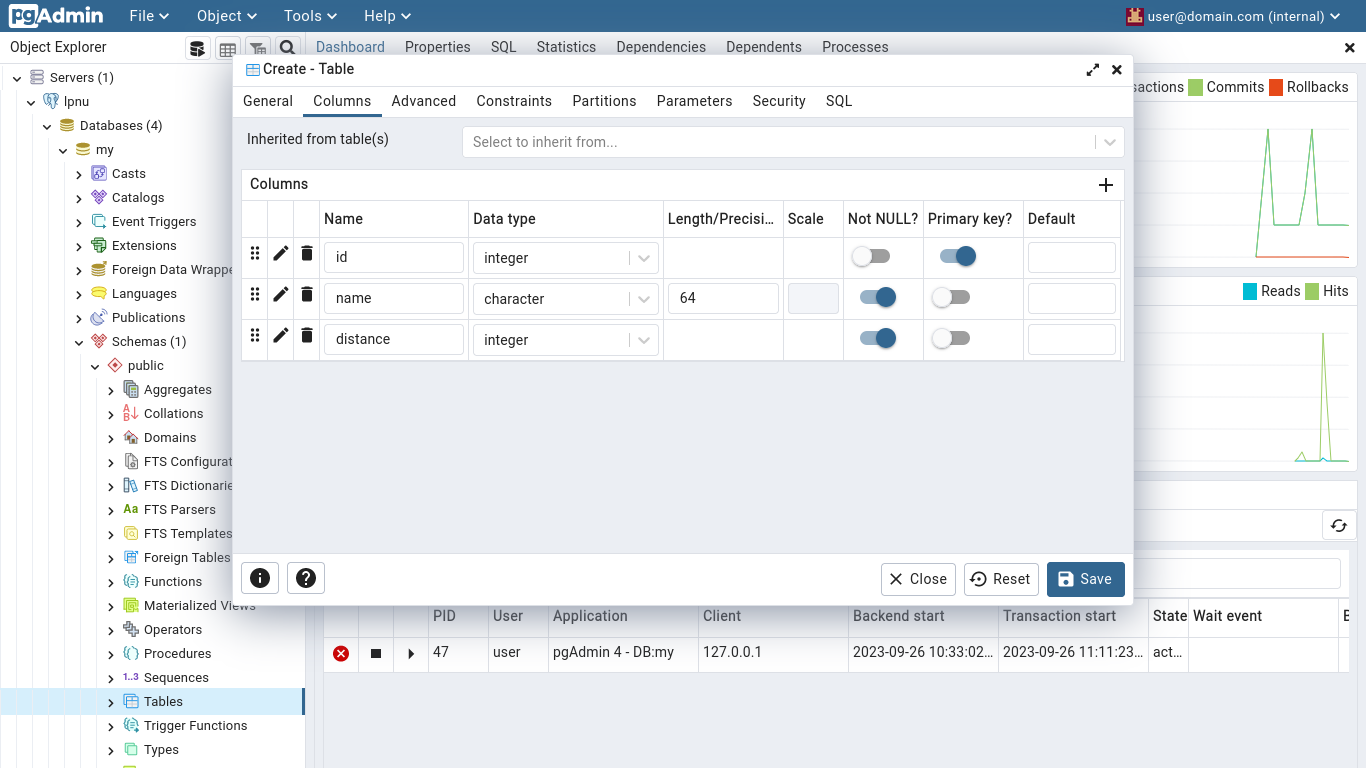
\includegraphics[scale=0.35]{21}
		\caption{Створення таблиці "route"}
	\end{figure}

	\begin{figure}[H]
		\centering
		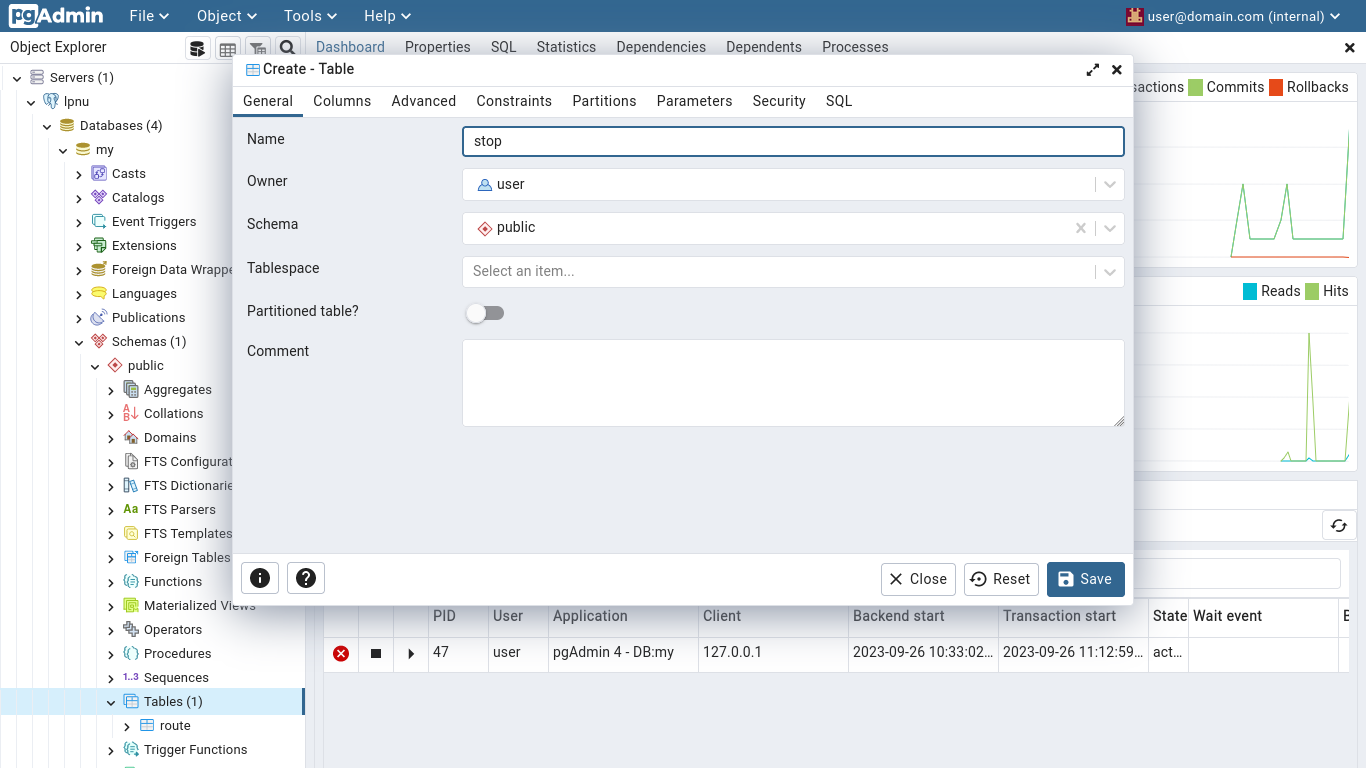
\includegraphics[scale=0.35]{22}
		\caption{Створення таблиці "stop"}
	\end{figure}
	
	\begin{figure}[H]
		\centering
		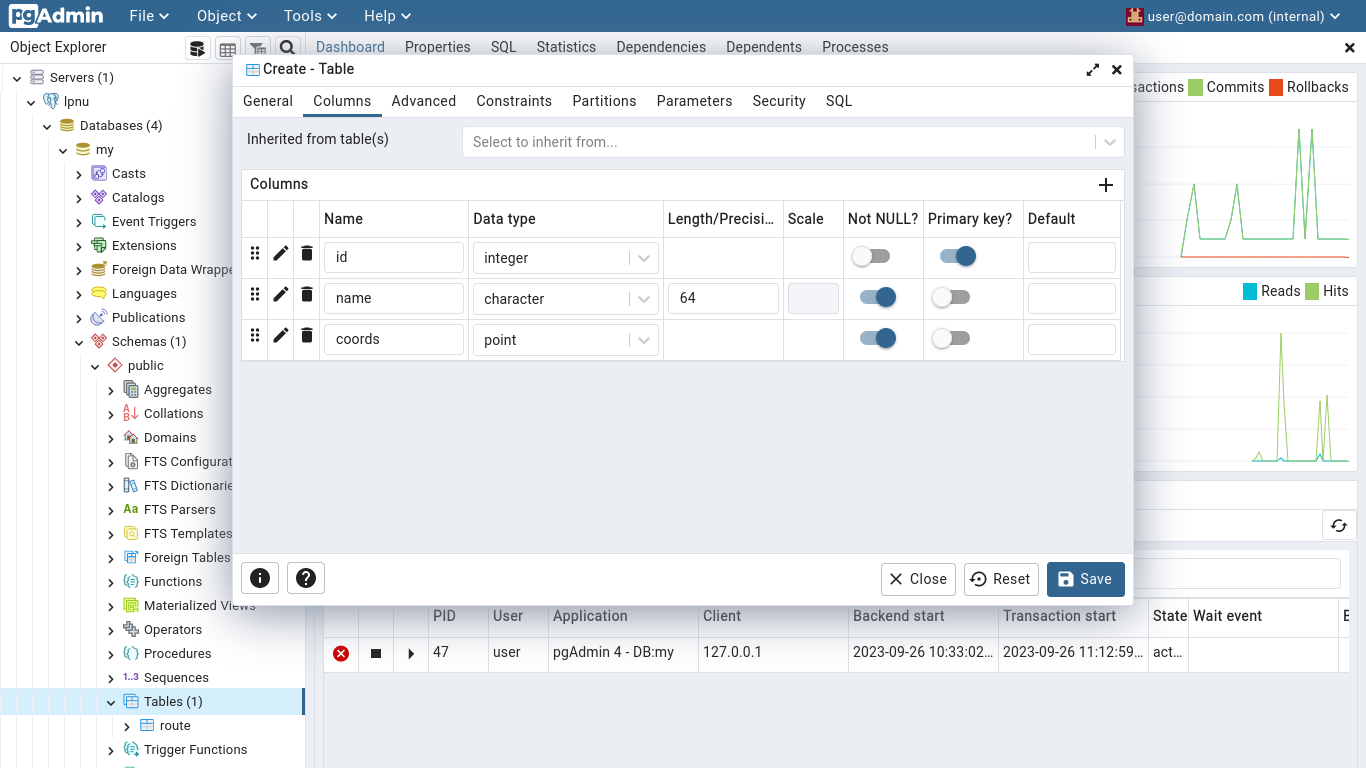
\includegraphics[scale=0.35]{23}
		\caption{Створення таблиці "stop"}
	\end{figure}

	\begin{figure}[H]
		\centering
		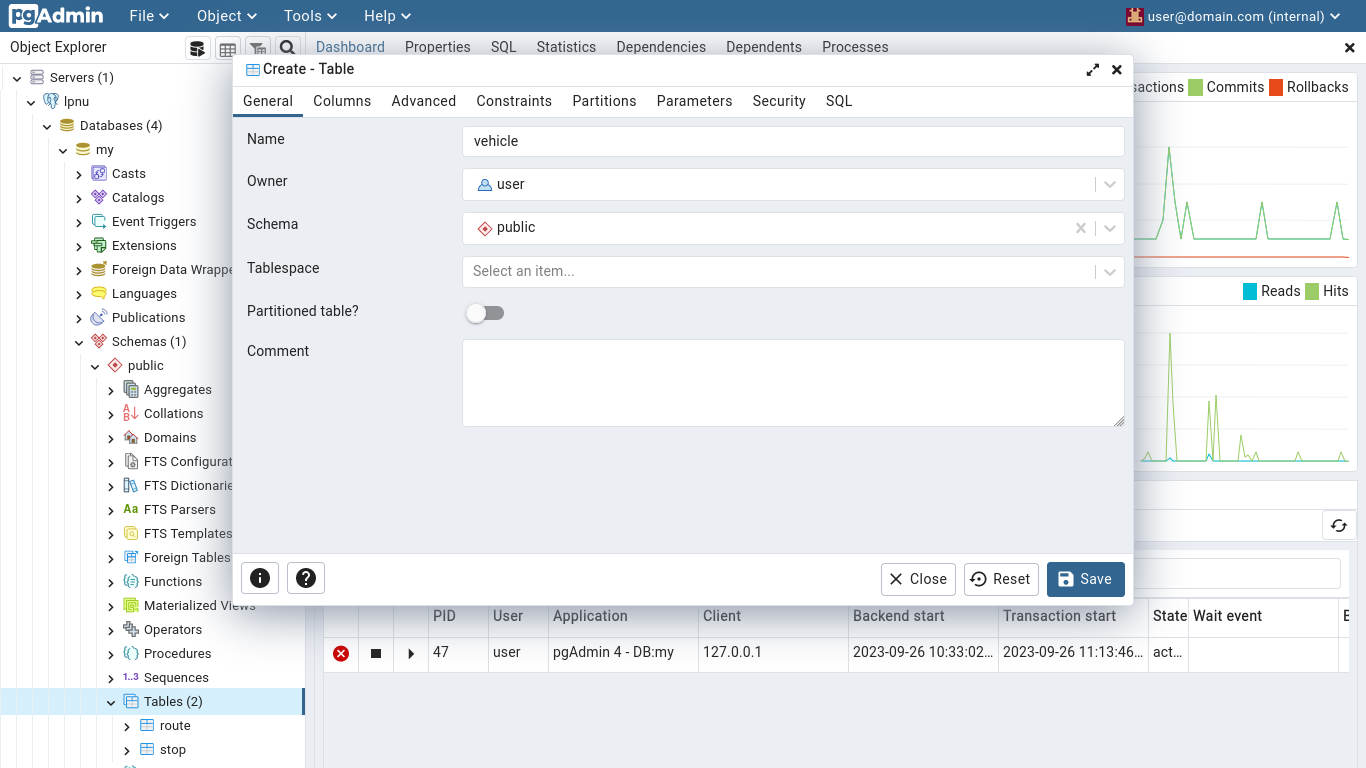
\includegraphics[scale=0.35]{24}
		\caption{Створення таблиці "vehicle"}
	\end{figure}
	
	\begin{figure}[H]
		\centering
		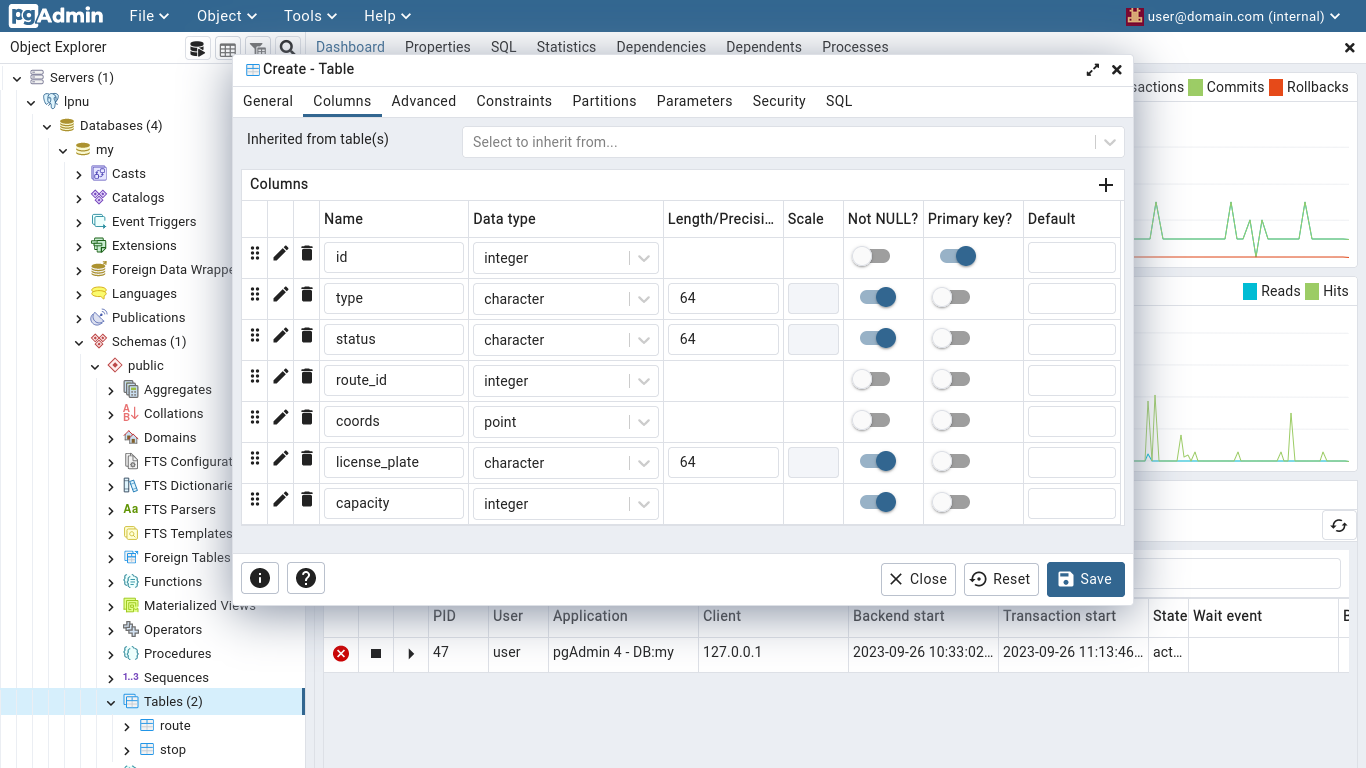
\includegraphics[scale=0.35]{25}
		\caption{Створення таблиці "vehicle"}
	\end{figure}
	
	\begin{figure}[H]
		\centering
		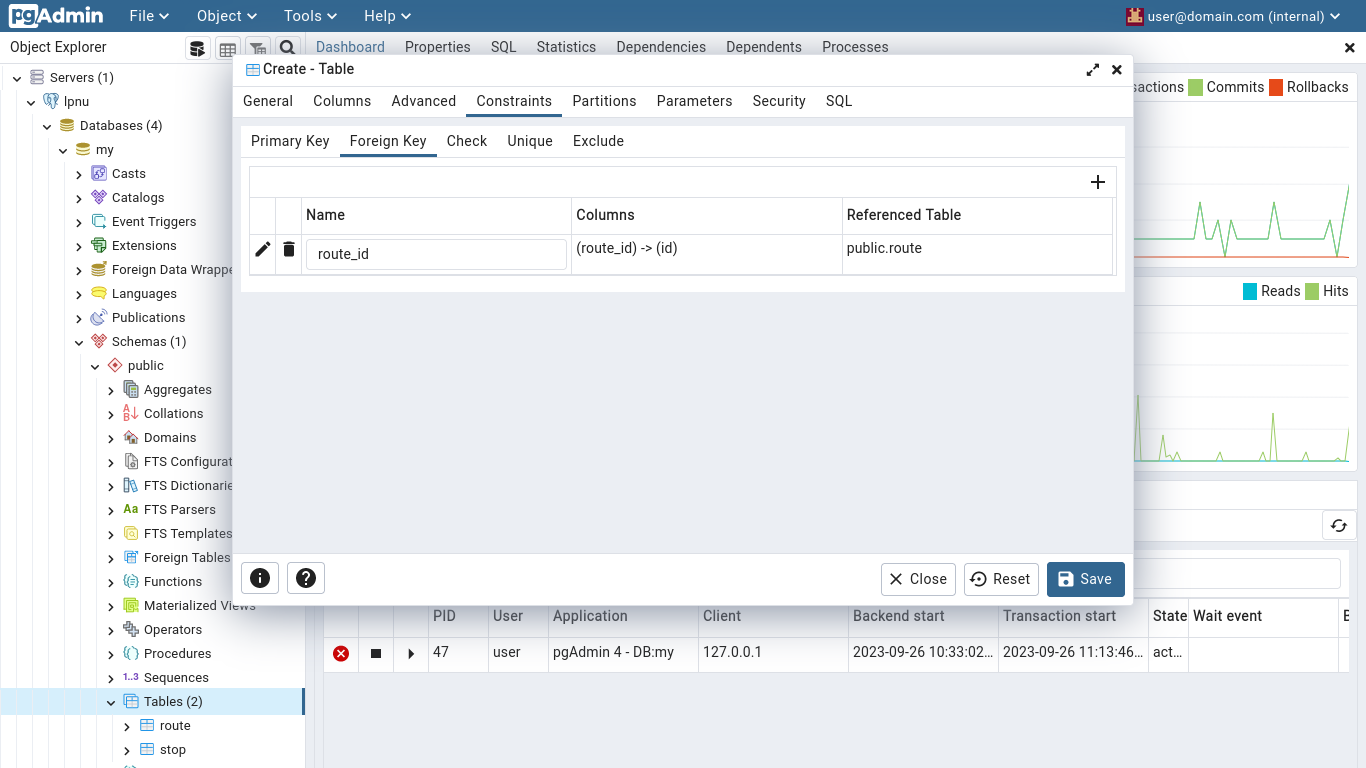
\includegraphics[scale=0.35]{26}
		\caption{Створення таблиці "vehicle"}
	\end{figure}
	
	\begin{figure}[H]
		\centering
		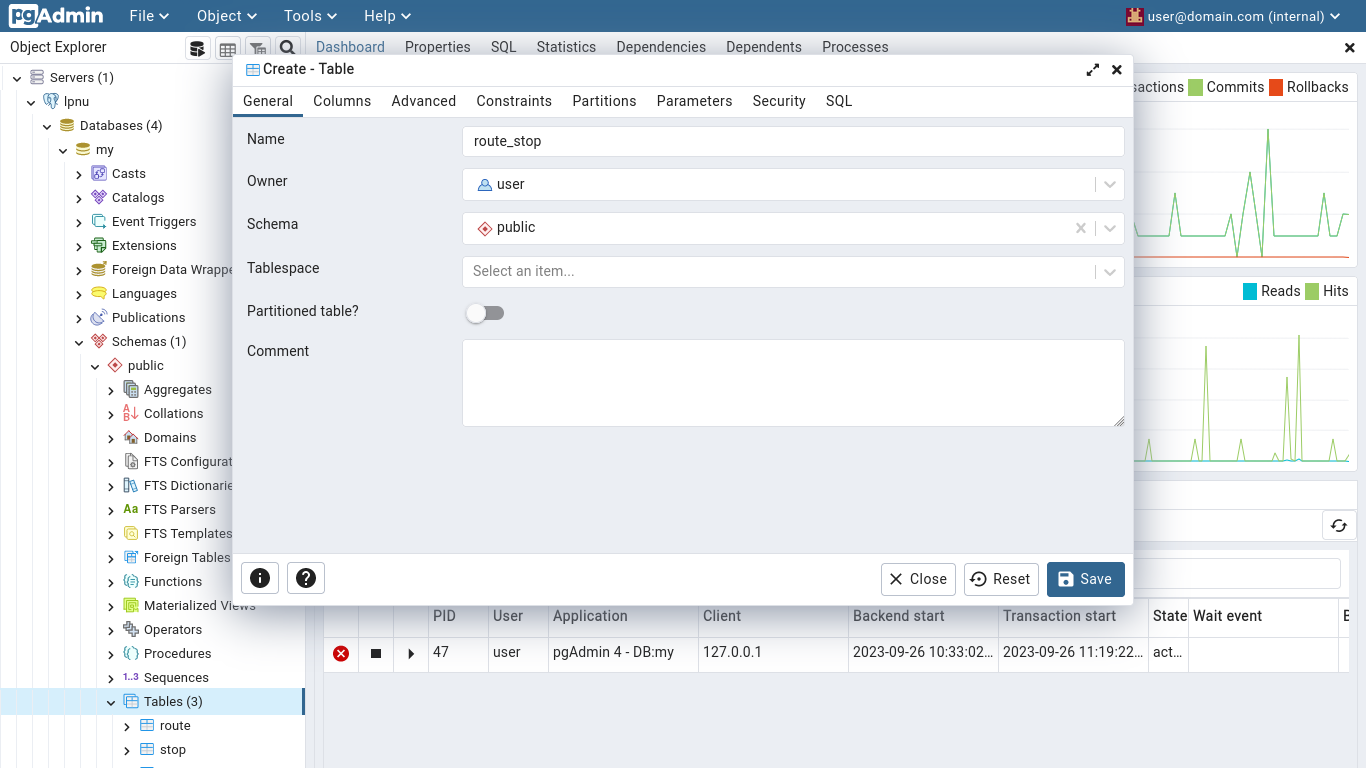
\includegraphics[scale=0.35]{27}
		\caption{Створення таблиці "route\_stop"}
	\end{figure}
	
	\begin{figure}[H]
		\centering
		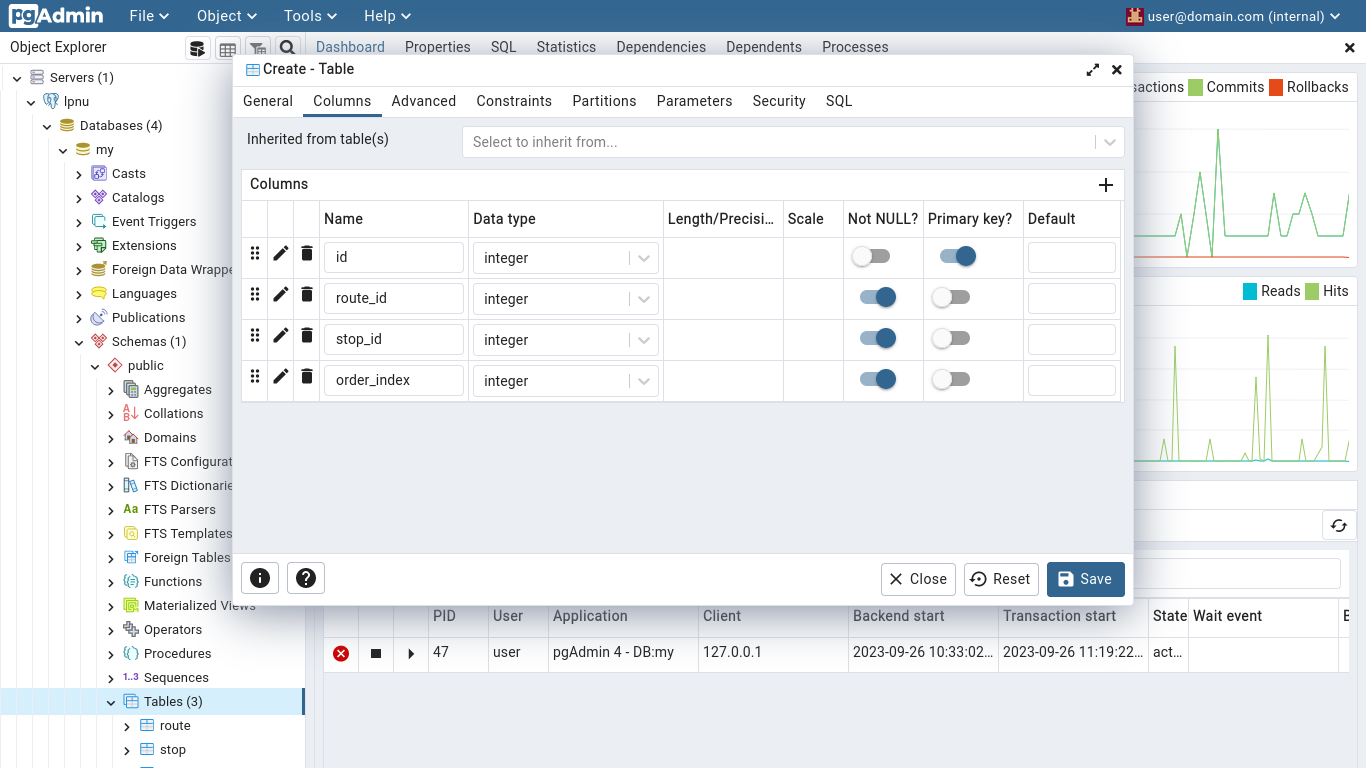
\includegraphics[scale=0.35]{28}
		\caption{Створення таблиці "route\_stop}
	\end{figure}
	
	\begin{figure}[H]
		\centering
		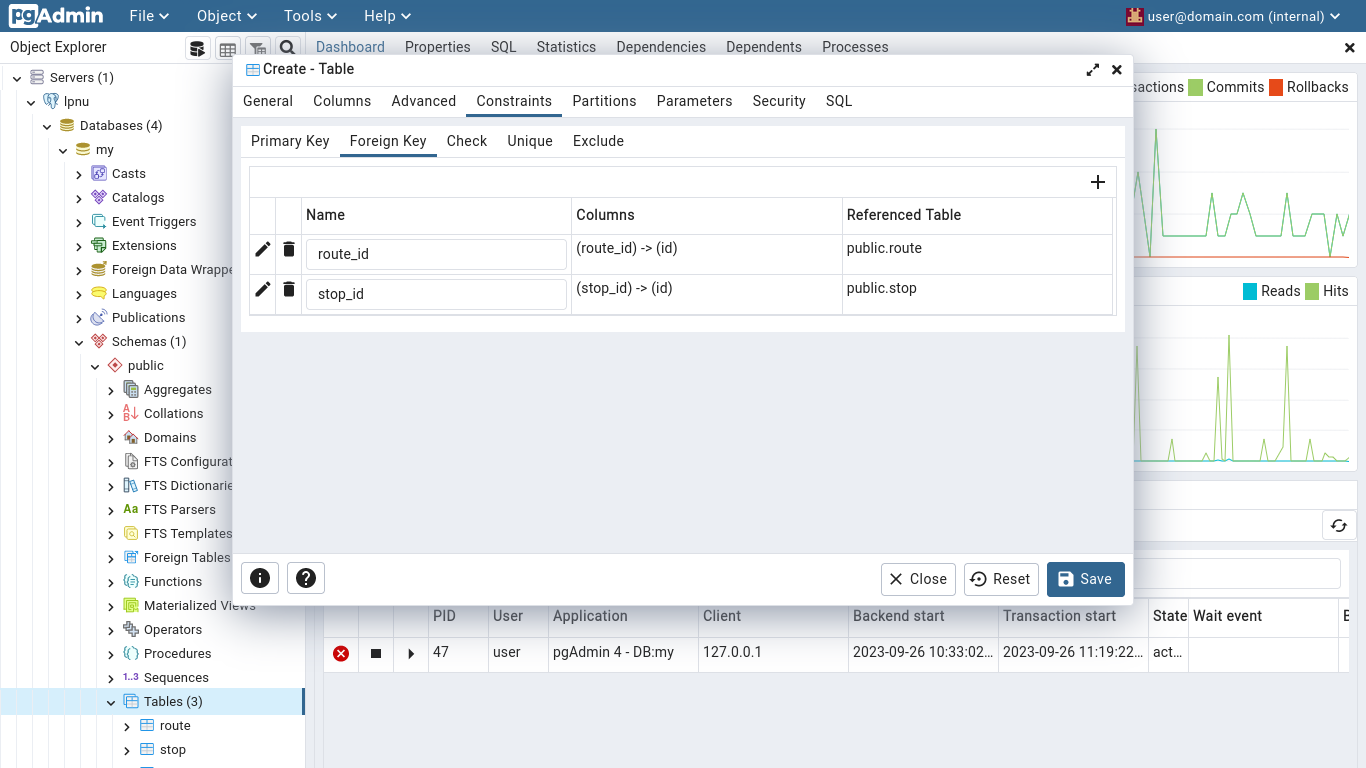
\includegraphics[scale=0.35]{29}
		\caption{Створення таблиці "route\_stop"}
	\end{figure}
	
	\begin{figure}[H]
		\centering
		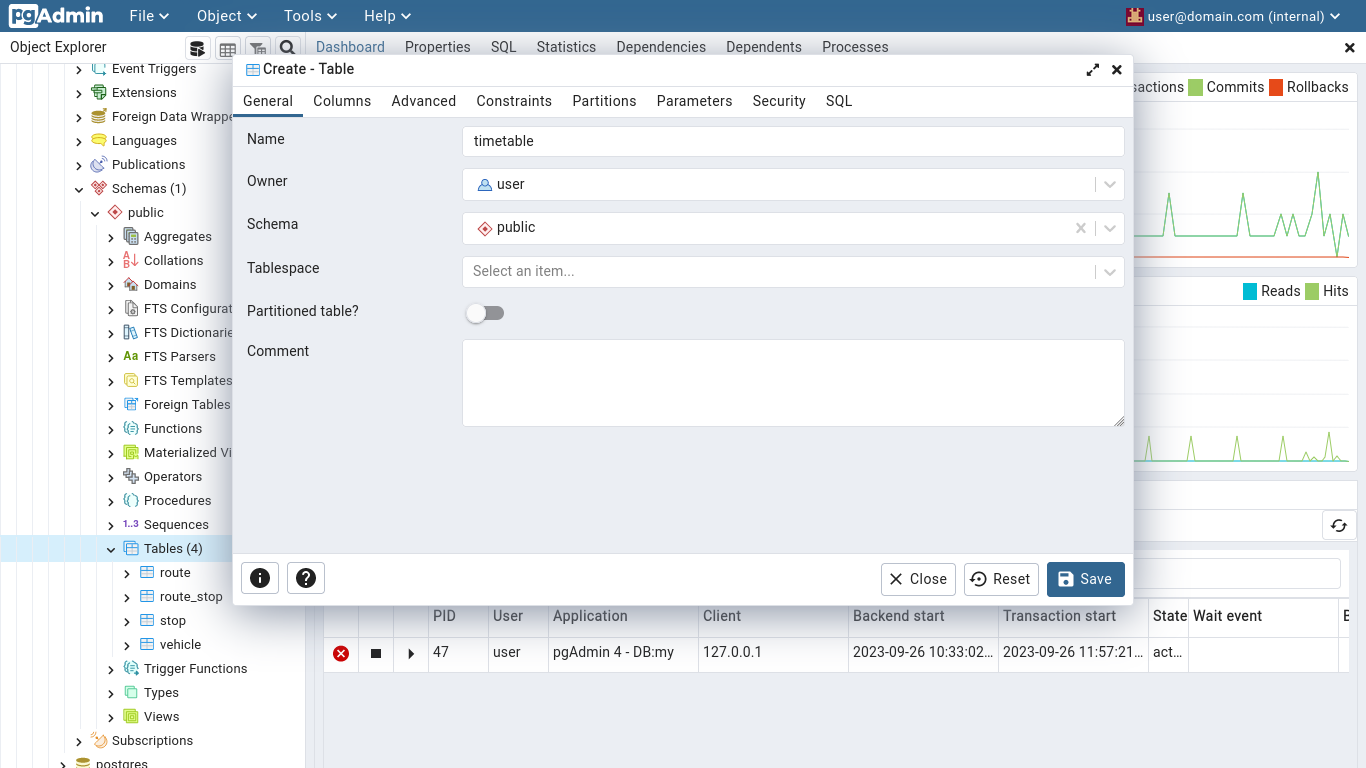
\includegraphics[scale=0.35]{30}
		\caption{Створення таблиці "timetable"}
	\end{figure}
	
	\begin{figure}[H]
		\centering
		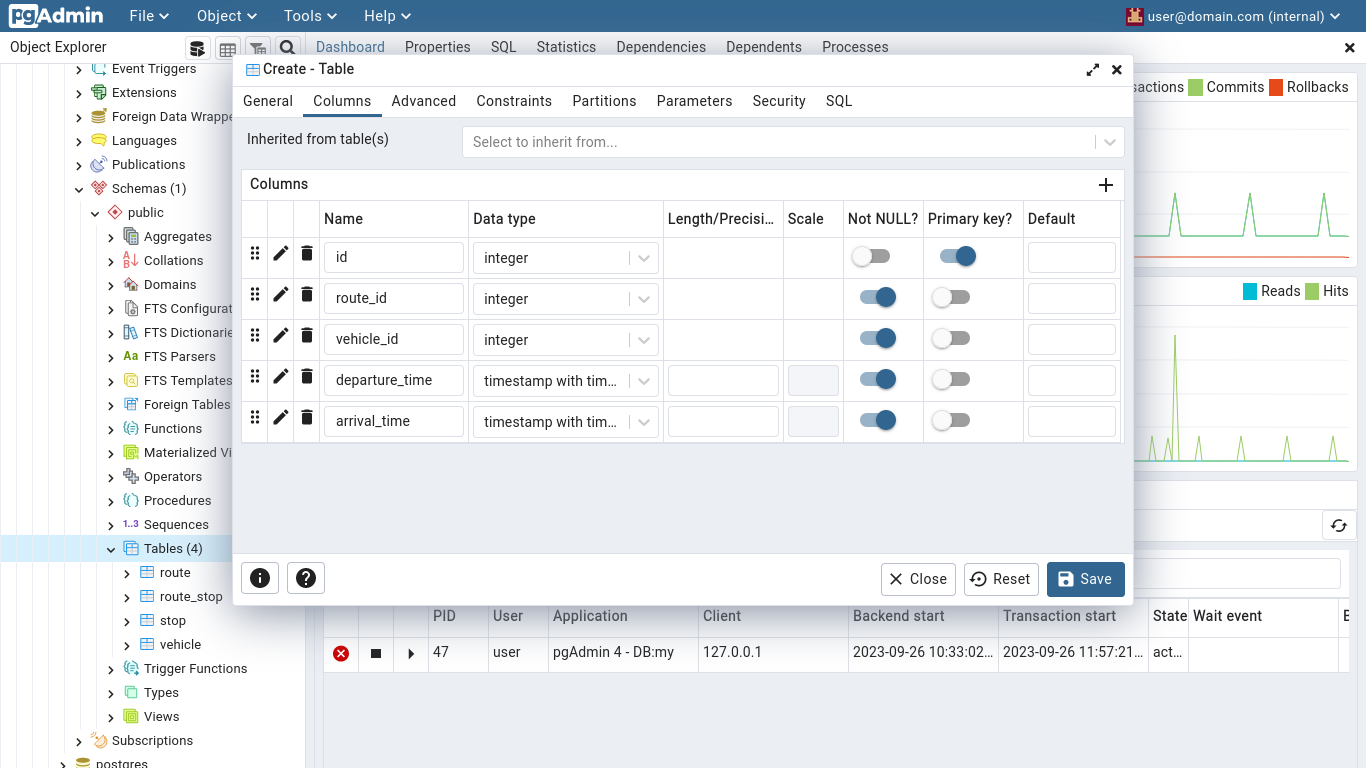
\includegraphics[scale=0.35]{31}
		\caption{Створення таблиці "timetable}
	\end{figure}
	
	\begin{figure}[H]
		\centering
		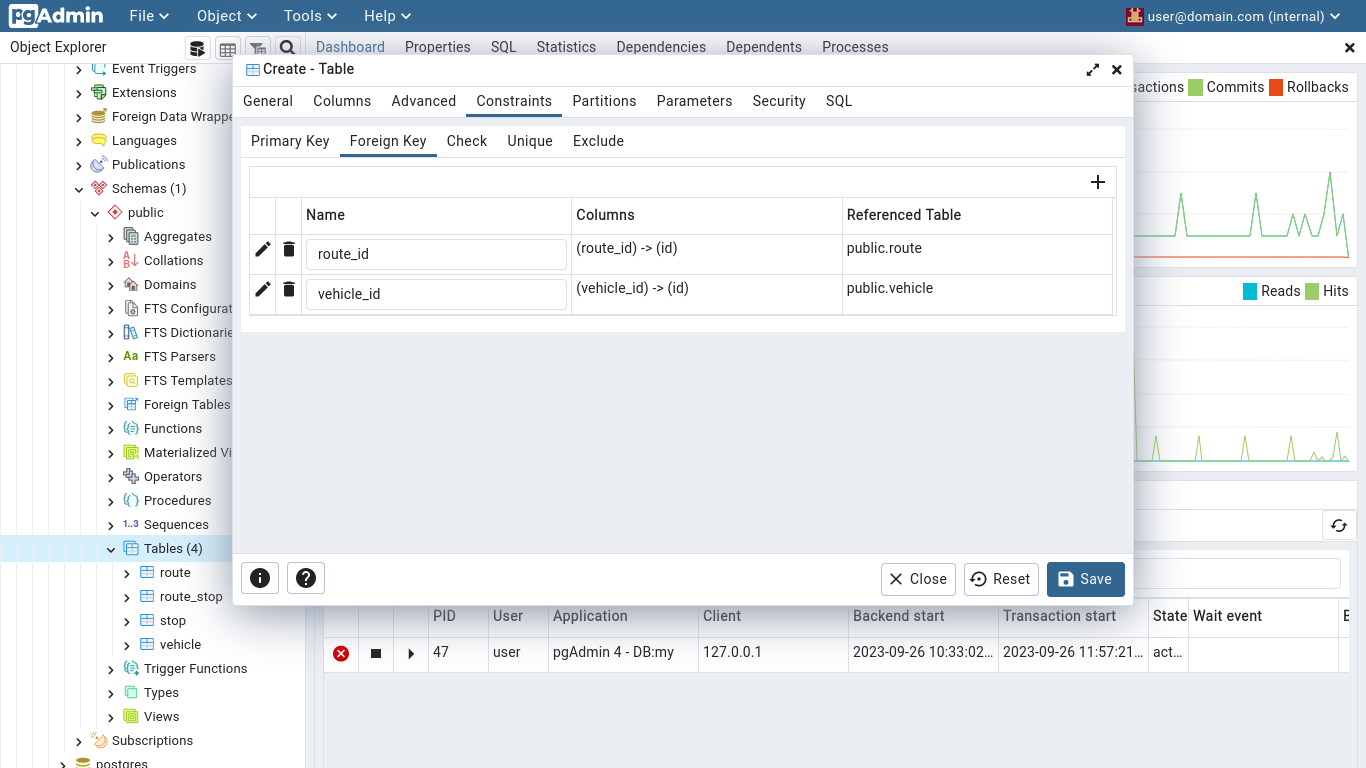
\includegraphics[scale=0.35]{32}
		\caption{Створення таблиці "timetable"}
	\end{figure}
	
	\begin{figure}[H]
		\centering
		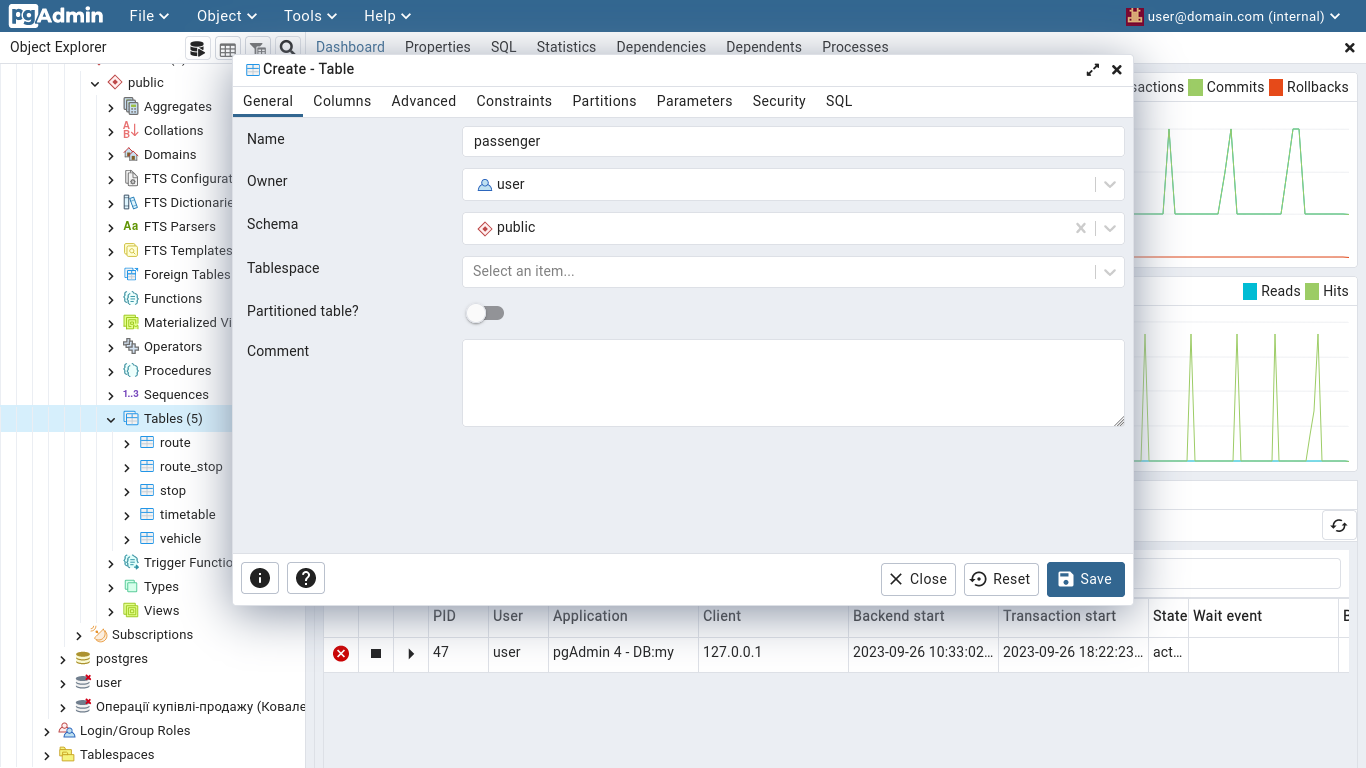
\includegraphics[scale=0.35]{33}
		\caption{Створення таблиці "passenger"}
	\end{figure}
	
	\begin{figure}[H]
		\centering
		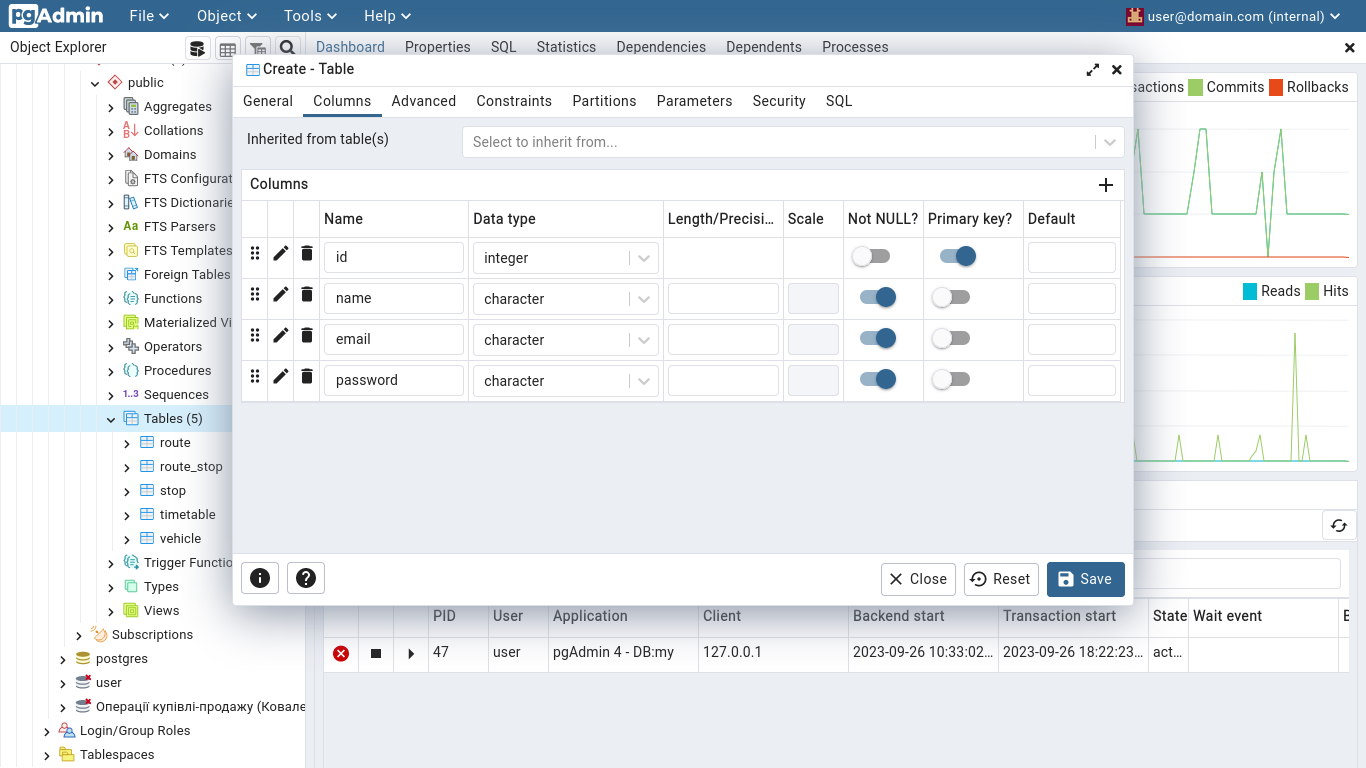
\includegraphics[scale=0.35]{34}
		\caption{Створення таблиці "passenger}
	\end{figure}
	
	\begin{figure}[H]
		\centering
		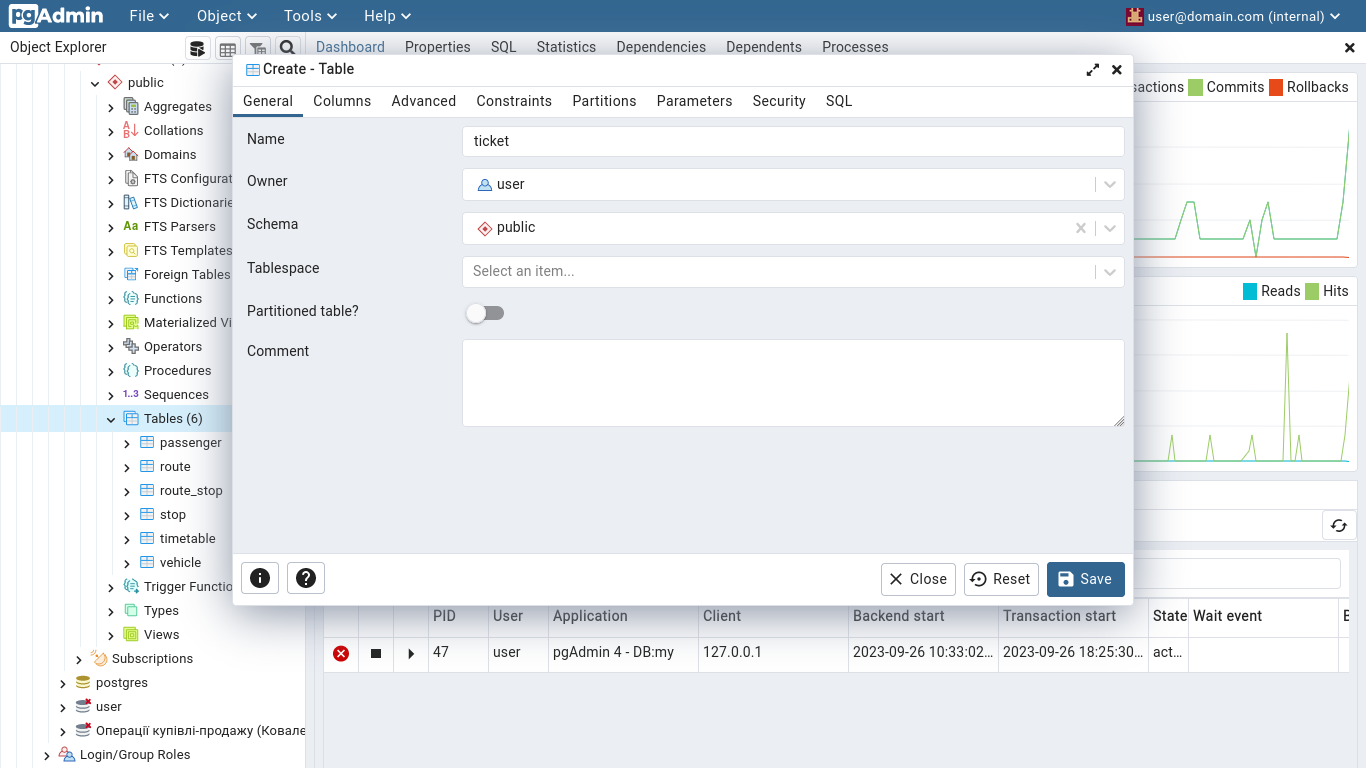
\includegraphics[scale=0.35]{35}
		\caption{Створення таблиці "ticket"}
	\end{figure}
	
	\begin{figure}[H]
		\centering
		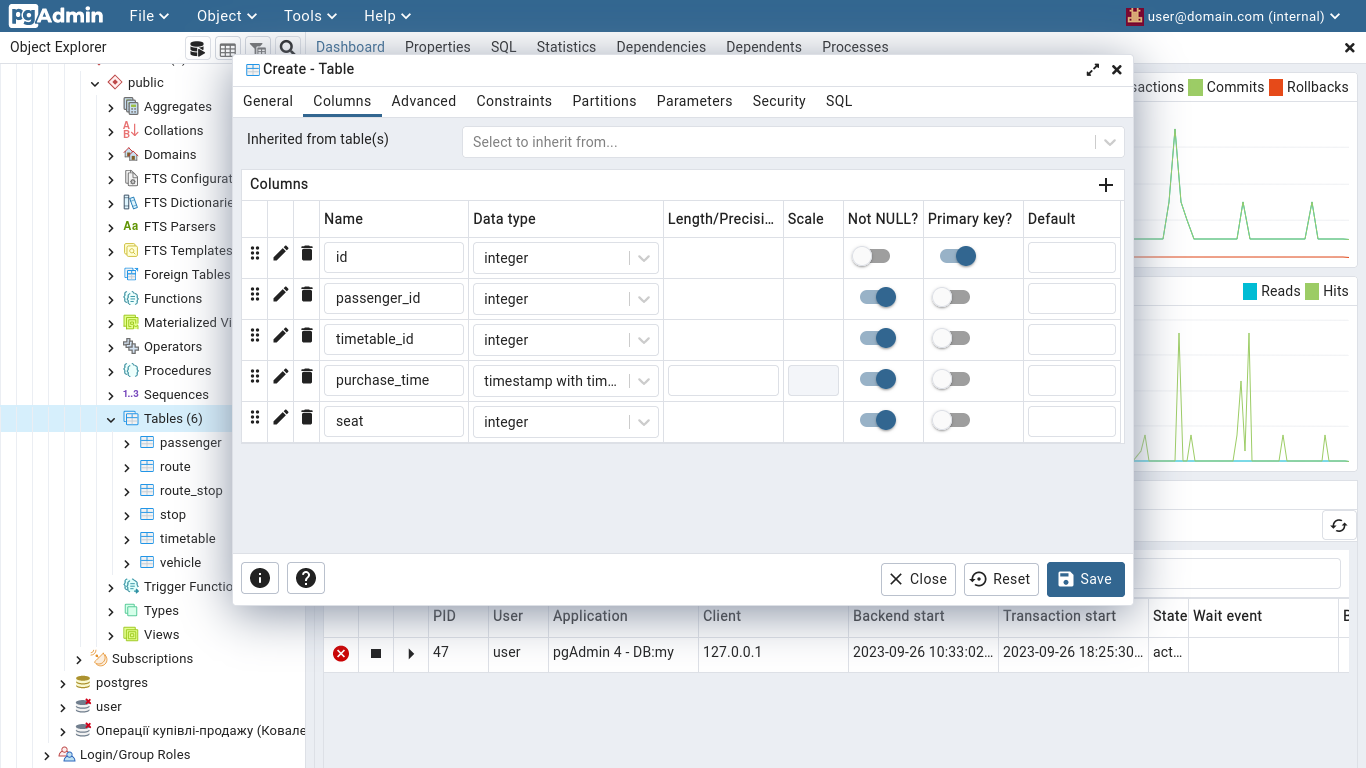
\includegraphics[scale=0.35]{36}
		\caption{Створення таблиці "ticket}
	\end{figure}
	
	\begin{figure}[H]
		\centering
		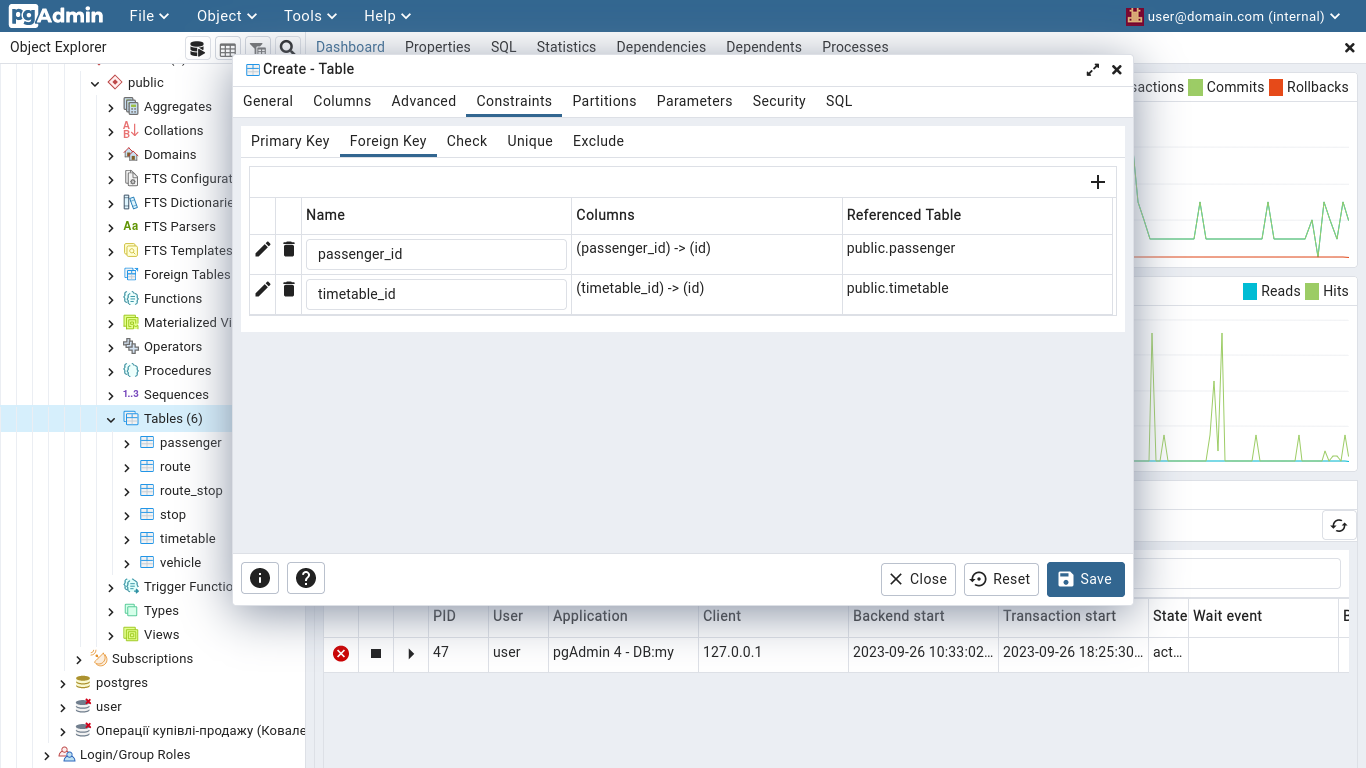
\includegraphics[scale=0.35]{37}
		\caption{Створення таблиці "ticket"}
	\end{figure}
	
	\begin{figure}[H]
		\centering
		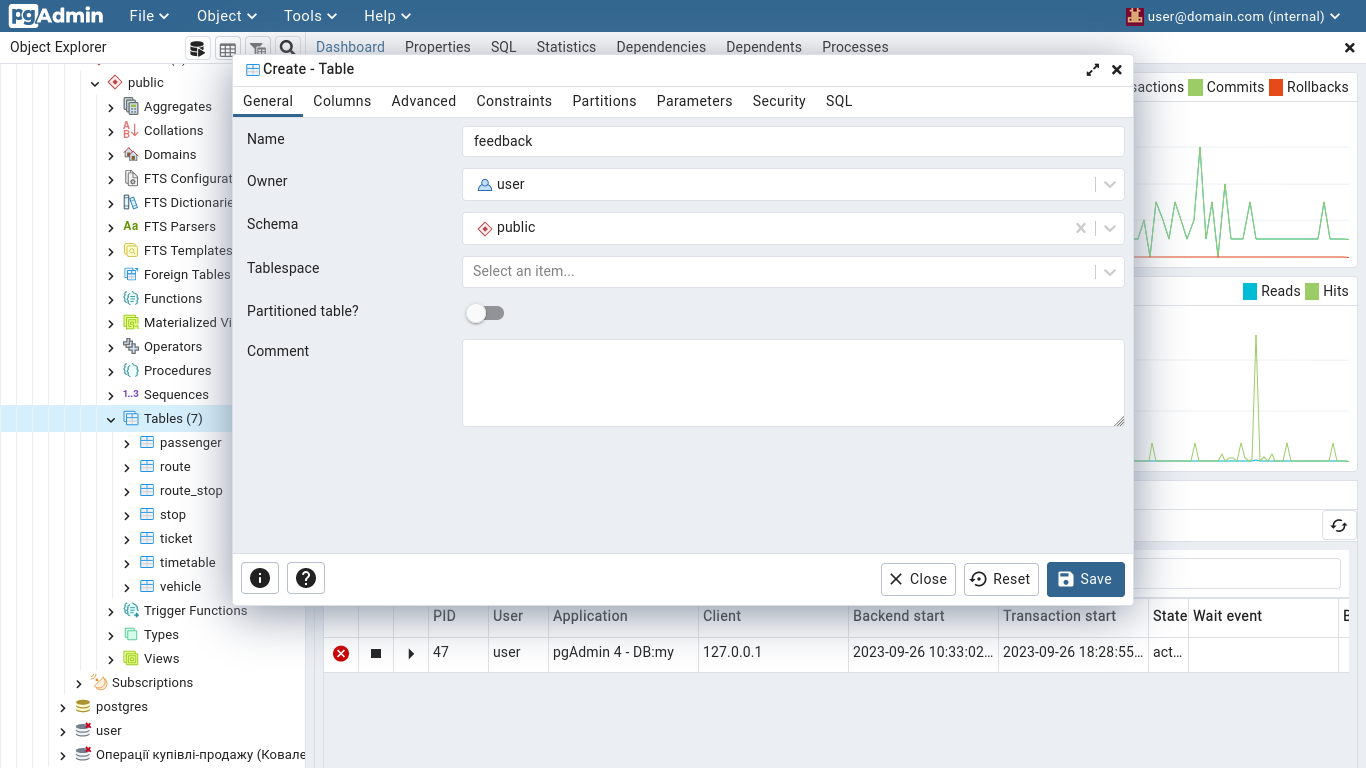
\includegraphics[scale=0.35]{38}
		\caption{Створення таблиці "feedback"}
	\end{figure}
	
	\begin{figure}[H]
		\centering
		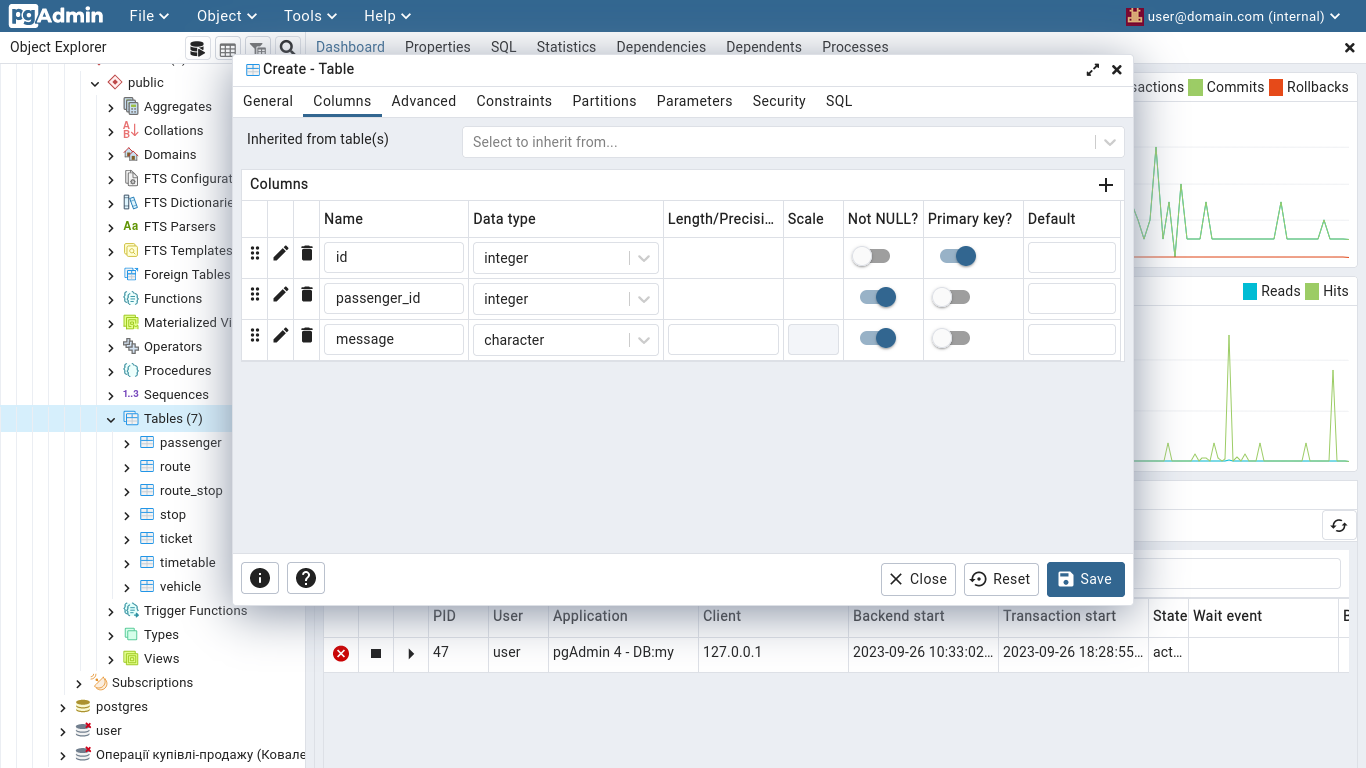
\includegraphics[scale=0.35]{39}
		\caption{Створення таблиці "feedback}
	\end{figure}
	
	\begin{figure}[H]
		\centering
		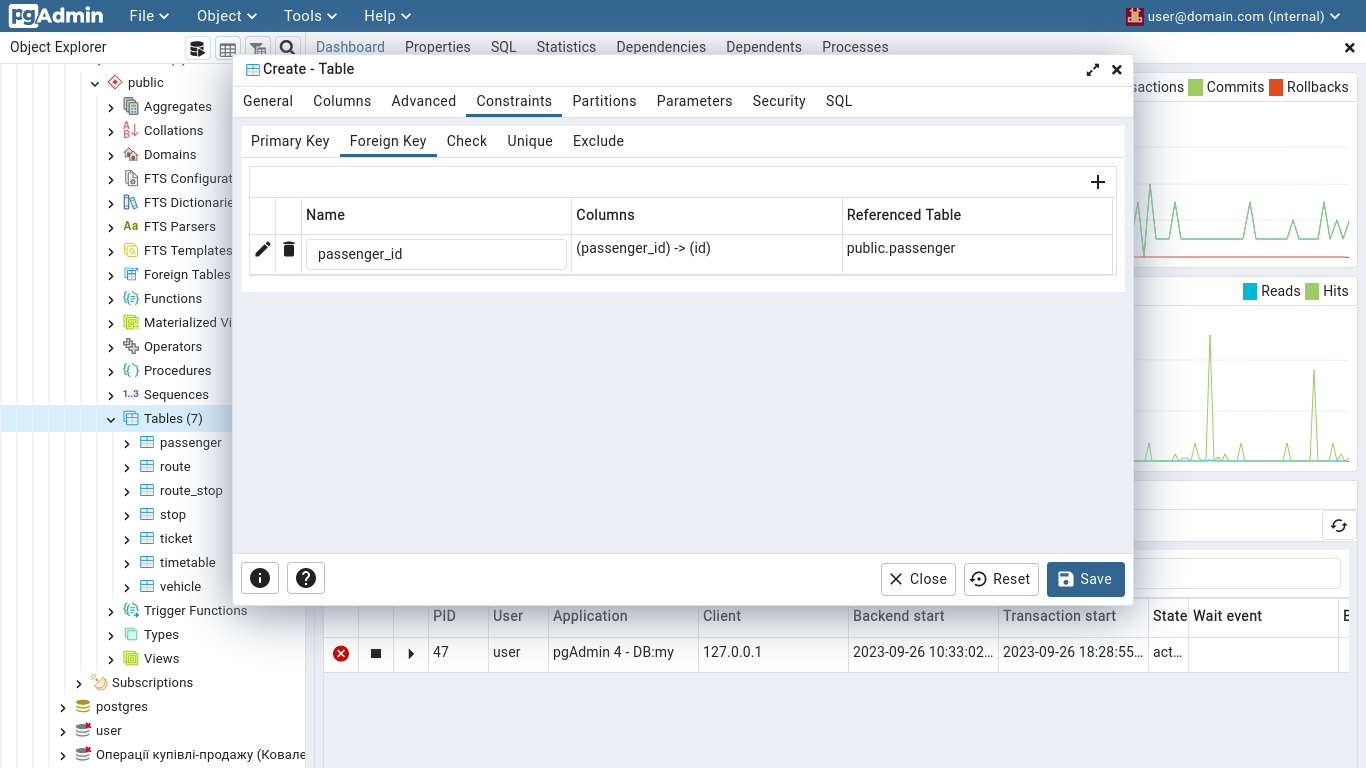
\includegraphics[scale=0.35]{40}
		\caption{Створення таблиці "feedback"}
	\end{figure}
	
	\begin{figure}[H]
		\centering
		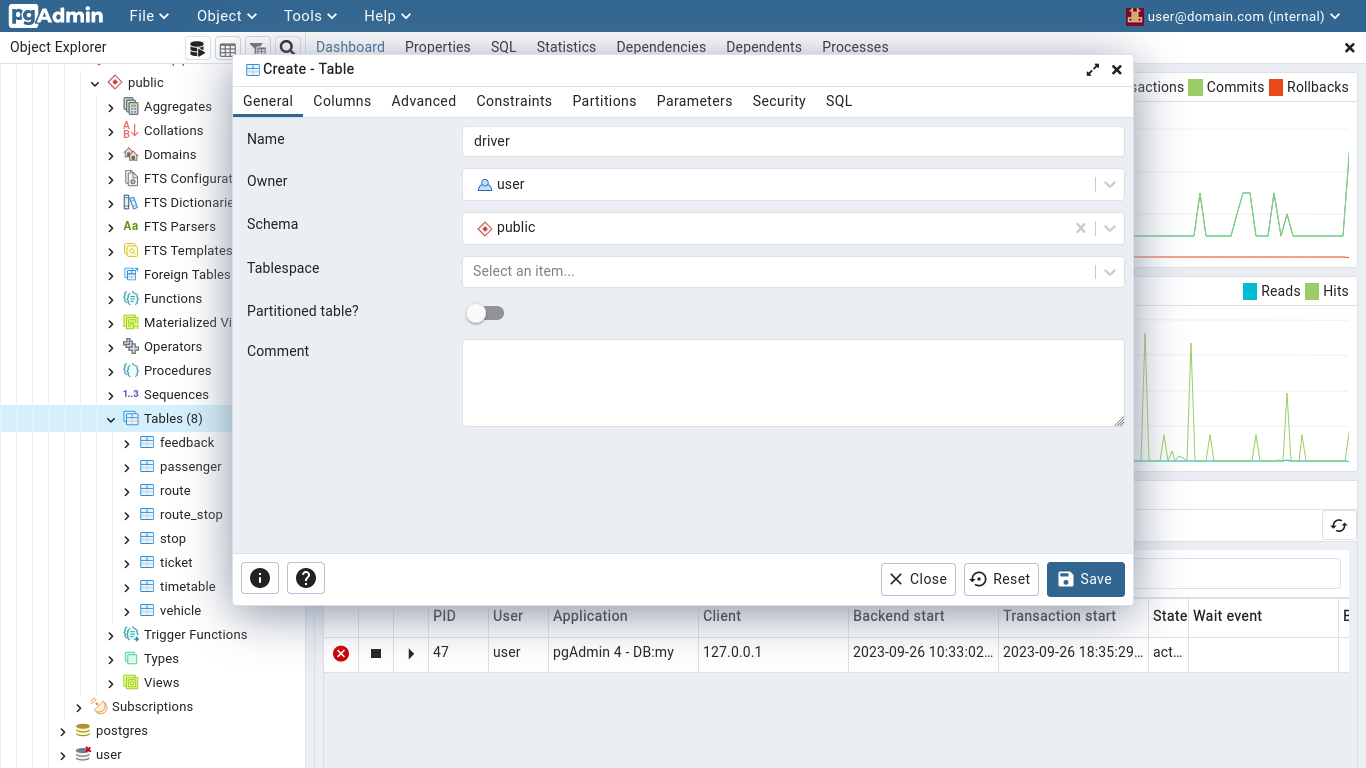
\includegraphics[scale=0.35]{41}
		\caption{Створення таблиці "driver"}
	\end{figure}
	
	\begin{figure}[H]
		\centering
		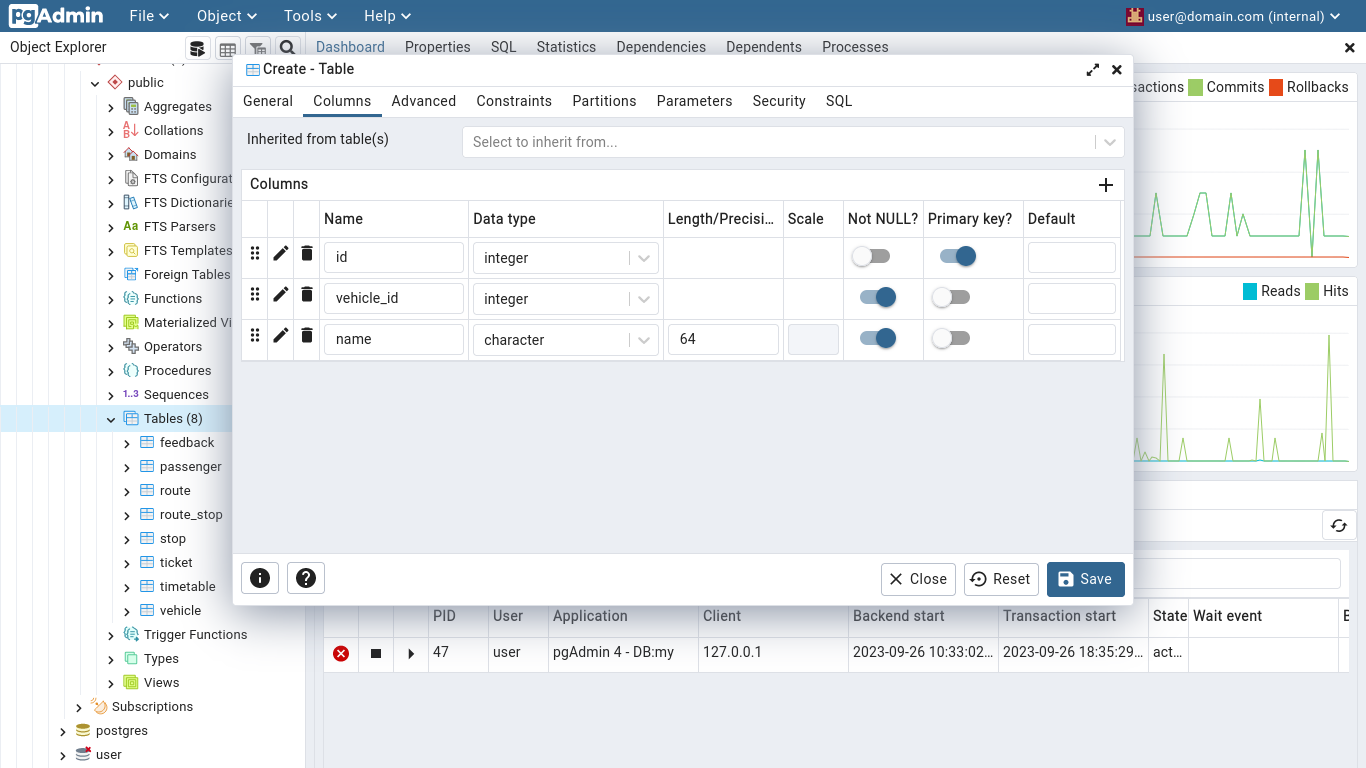
\includegraphics[scale=0.35]{42}
		\caption{Створення таблиці "driver}
	\end{figure}
	
	\begin{figure}[H]
		\centering
		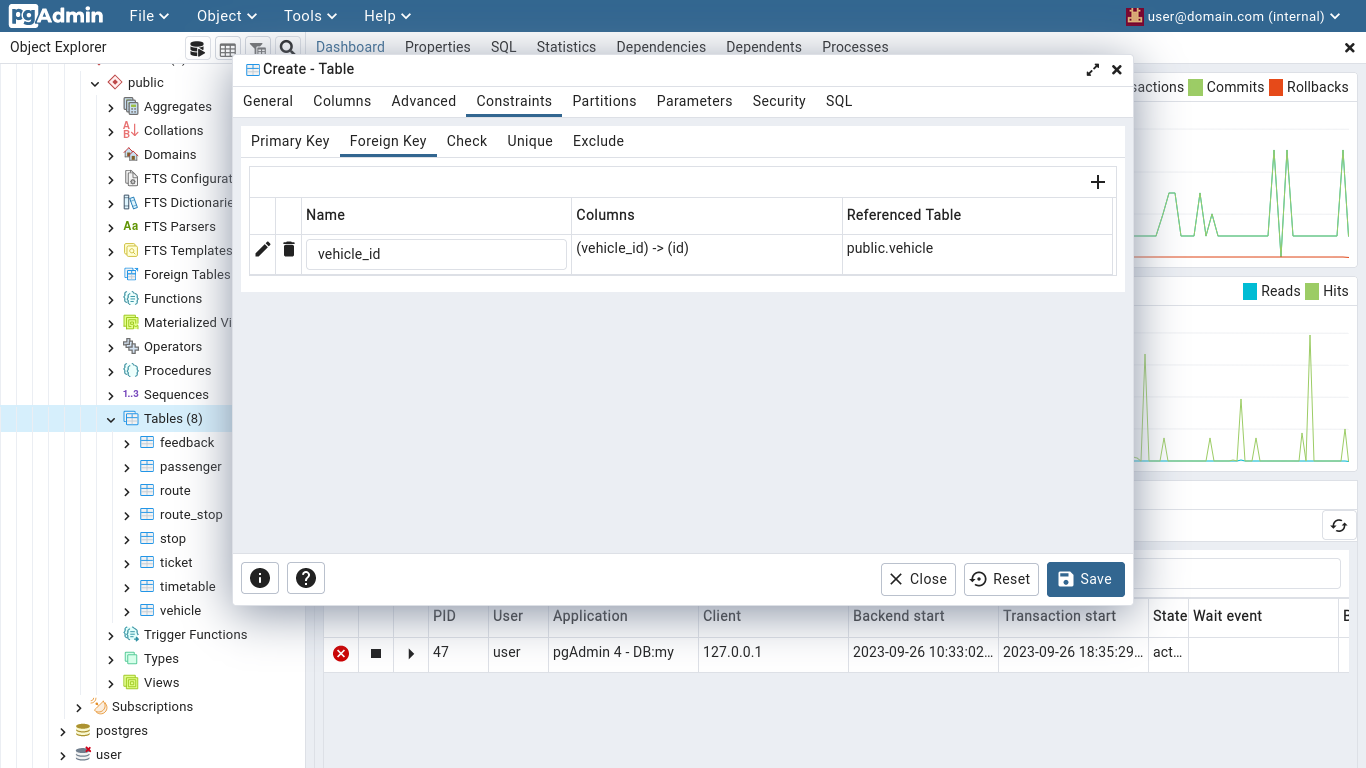
\includegraphics[scale=0.35]{43}
		\caption{Створення таблиці "driver"}
	\end{figure}
	
	\begin{figure}[H]
		\centering
		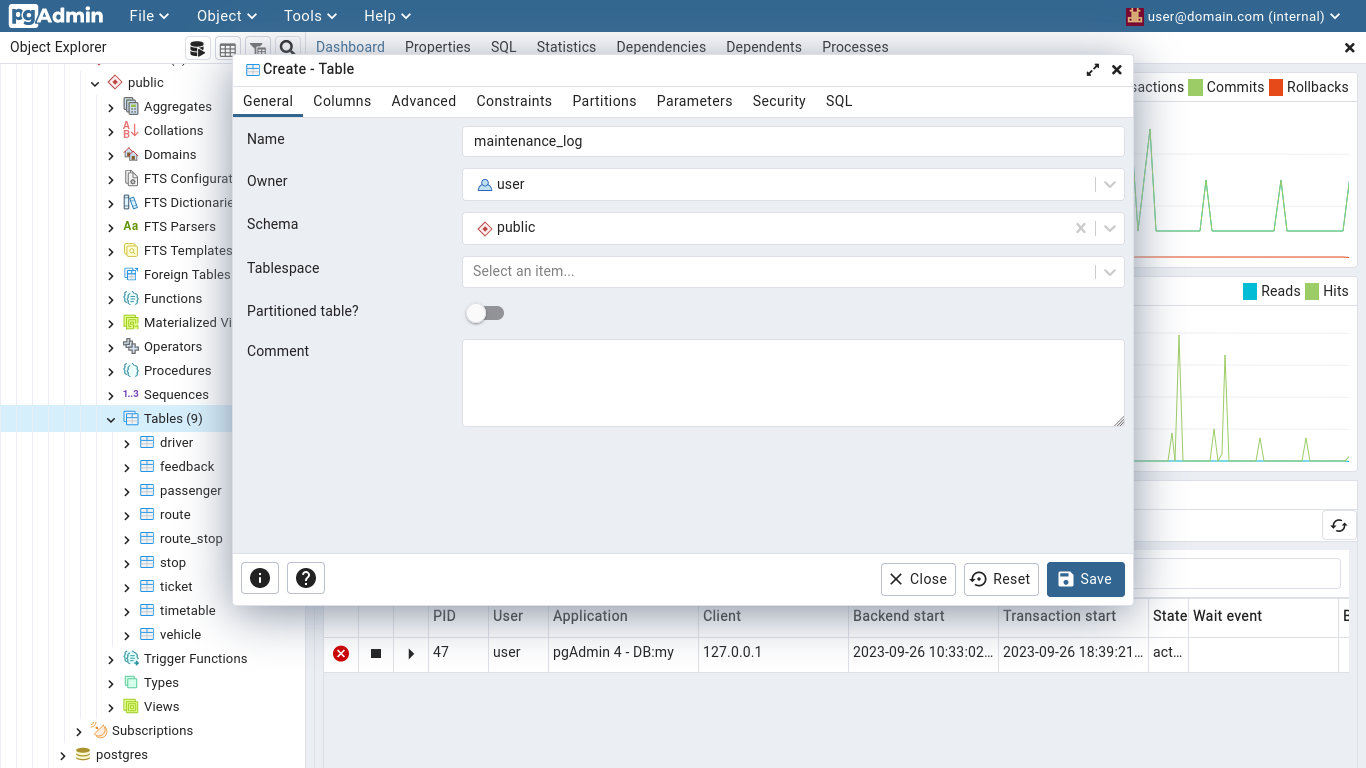
\includegraphics[scale=0.35]{44}
		\caption{Створення таблиці "maintenance\_log"}
	\end{figure}
	
	\begin{figure}[H]
		\centering
		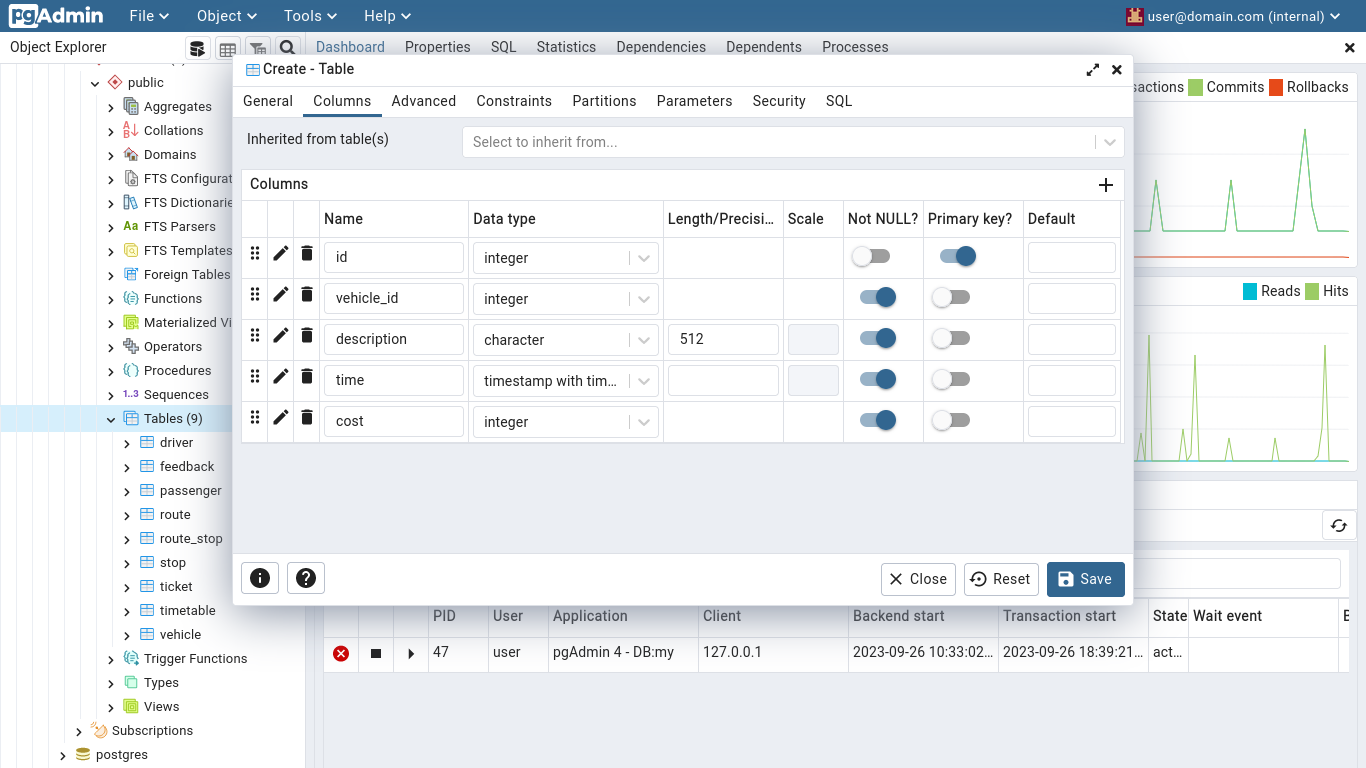
\includegraphics[scale=0.35]{45}
		\caption{Створення таблиці "maintenance\_log}
	\end{figure}
	
	\begin{figure}[H]
		\centering
		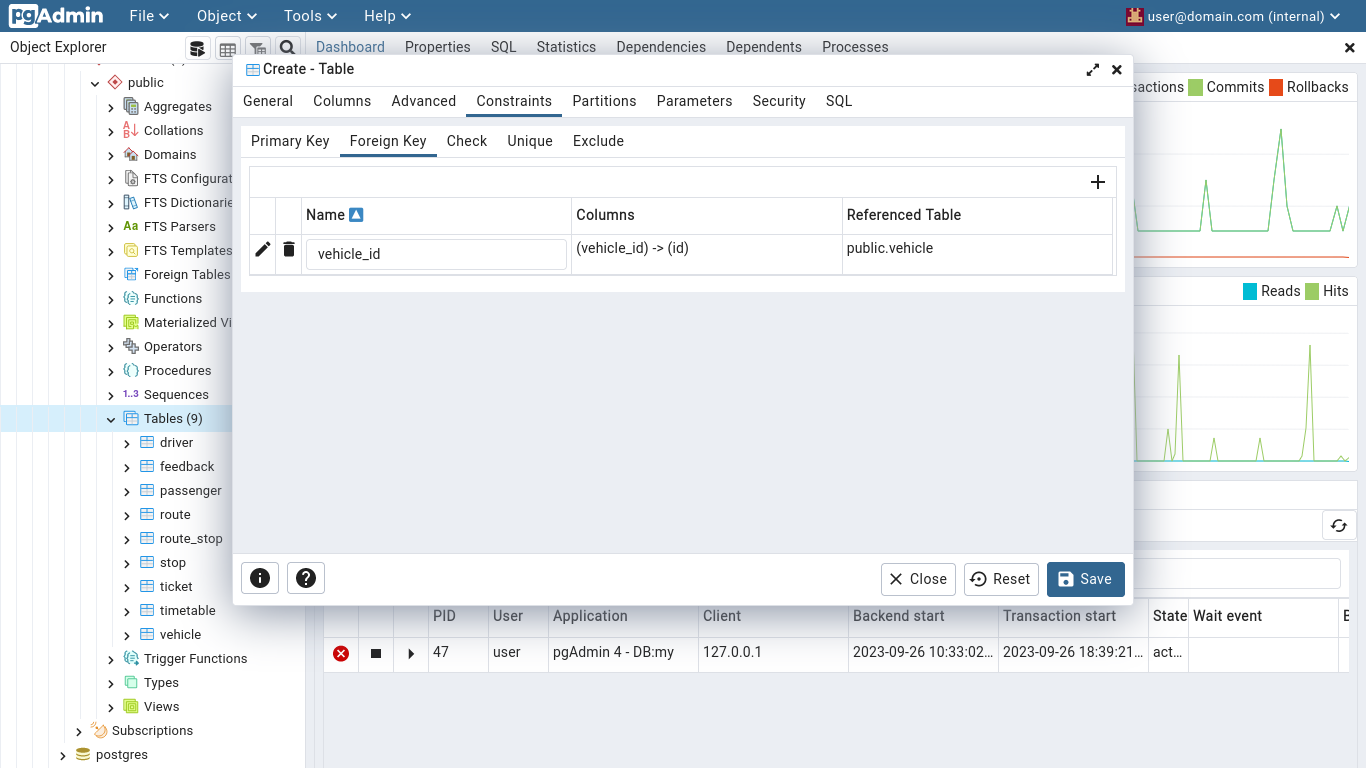
\includegraphics[scale=0.35]{46}
		\caption{Створення таблиці "maintenance\_log"}
	\end{figure}
	\fi
	\section*{Висновок}
	Під час виконання лабораторної роботи я встановив та налаштував PostgreSQL та PgAdmin. Для виконання лабораторної роботи я обрав шлях для встановлення та налаштування необхідних програмних компонентів за допомогою контейнеризованого оточення. Я здобув необхідні навички для роботи з PostgreSQL та pgAdmin.
	 
\end{normalsize}
\end{document}
